% Created 2018-06-01 Fri 14:47
% Intended LaTeX compiler: pdflatex
\documentclass[11pt]{book}
\usepackage[utf8]{inputenc}
\usepackage[T1]{fontenc}
\usepackage{graphicx}
\usepackage{grffile}
\usepackage{longtable}
\usepackage{wrapfig}
\usepackage{rotating}
\usepackage[normalem]{ulem}
\usepackage{amsmath}
\usepackage{textcomp}
\usepackage{amssymb}
\usepackage{capt-of}
\usepackage{hyperref}
\usepackage{amsthm}
\usepackage{amsmath,amscd,amssymb,mathtools}
\usepackage{tikz-cd}
\usepackage{svg}
\usepackage[all]{xy}
\usepackage{pgfplots}
\newtheorem{remark}{Remark}
\newtheorem{theorem}{Theorem}
\newtheorem{lemma}[theorem]{Lemma}
\newtheorem{corollary}{Corollary}[theorem]
\newtheorem{conjecture}[theorem]{Conjecture}
\newtheorem{proposition}{Proposition}[theorem]
\newtheorem{problem}{Problem}
\newtheorem{exampl}{Example}
\newtheorem{definition}{Definition}
\newtheorem{propdef}[definition]{Proposition-Definition}
\newcommand{\re}{\mathop{\rm Re}\nolimits}
\newcommand{\im}{\mathop{\rm Im}\nolimits}
\newcommand{\coker}{\mathop{\rm coker}\nolimits}
\newcommand{\supp}{\mathop{\rm supp}\nolimits}
\newcommand{\ord}{\mathop{\rm ord}\nolimits}
\newcommand{\Spec}{\mathop{\rm Spec}\nolimits}
\newcommand{\vol}{\mathop{\rm vol}\nolimits}
\newcommand*{\transp}[2][-3mu]{\ensuremath{\mskip1mu\prescript{\smash{\mathrm t\mkern#1}}{}{\mathstrut#2}}}
\newcommand{\sff}{\mathop{\rm I\*I}\nolimits}
\newcommand{\tr}{\mathop{\rm Tr}\nolimits}
\newcommand{\const}{\mathop{\rm const }\nolimits}
\newcommand{\lcm}{\mathop{\rm lcm}\nolimits}
%\newcommand{\gcd}{\mathop{\rm gcd}\nolimits}
\newcommand{\Ric}{\mathop{\rm Ric}\nolimits}
\newcommand{\Riem}{\mathop{\rm Riem}\nolimits}
\newcommand\restr[2]{{% we make the whole thing an ordinary symbol
\left.\kern-\nulldelimiterspace % automatically resize the bar with \right
#1 % the function
\vphantom{\big|} % pretend it's a little taller at normal size
\right|_{#2} % this is the delimiter
}}
\author{Tien NGUYEN MANH}
\date{June 1, 2018}
\title{Harmonic maps of Riemannian manifolds}
\hypersetup{
 pdfauthor={Tien NGUYEN MANH},
 pdftitle={Harmonic maps of Riemannian manifolds},
 pdfkeywords={},
 pdfsubject={},
 pdfcreator={Emacs 25.3.1 (Org mode 9.0.5)}, 
 pdflang={English}}
\begin{document}

\maketitle
\tableofcontents
\chapter{Summary}

The goal of this part is to give a summary of what will be developed in the next chapters. In brief, we are interested in
maps \(f: M \longrightarrow M'\) between Riemannian manifolds (that to simplify, are
supposed to be compact) that are critical points of the energy functional
\[
 E(f) = \frac{1}{2}\int_M |\nabla f|^2 dV
\]
that is, by taking first order variation of \(E\), those whose \textbf{tension field} \(\tau(f)\) vanish. 

We wish to prove that any smooth map \(f_0: M \longrightarrow M'\) can be deform to a
harmonic map using the gradient descent equation, that is to show the equation
\begin{equation}
\label{eq:intro:1}
\begin{cases}
\frac{df_t}{dt} = \tau(f_t)\\
\restr{f}{t=0} = f_0
\end{cases}
\end{equation}
We prove, in the rest of the memoire, that if \(M'\) is negatively curved then this PDE admits a globally defined smooth
solution \(f_t\) and that \(f_{\infty}:=\lim_{t\to \infty} f_t\) in \(C^\infty\) is
a harmonic map.

The resolution of \eqref{eq:intro:1} can be organised in 3 steps:
\begin{enumerate}
\item Find the global equation. We will find a global frame of \(M'\) and express
\(f\) in this frame, so that in stead of solving for a map, we will have to solve for functions.
\item Study linear PDEs on manifolds. The equation, expressed in local coordinates is a nonlinear heat equation, i.e. other
than a heat operator, it has a nonlinear differential operator of strictly lower
degree. Short-time existence and regularity for \eqref{eq:intro:1} follows from \emph{standard} results of
parabolic equation.
\item Prove long-time existence. This follows from several energy estimate.
\end{enumerate}

Local form of \eqref{eq:intro:1} can be found using calculus on Riemannian-connected vector
bundle. The relevant vector bundle here is \(f^* TM'\) over \(M\) in case of a single
map \(f: M \longrightarrow M'\), or \(F^* TM'\) over \(M\times[\alpha,\omega]\) for
a deformation \(F_t:\ M\times [\alpha,\omega] \longrightarrow M'\).

\section{Global equation.}
\label{sec:orgbbc11fd}

We will explain here how the step 1 is done. We will embed \(M'\) in a Euclidean space
\(\mathbb{R}^N\), not necessarily isometric because we will not use the Euclidean metric
on \(R^N\) anyway. We will equip a tubular neighborhood \(T\) of \(M'\), which is
diffeomorphic to \(M'\times D\) where \(D\) is an open disc of dimension equal the
codimension of \(M'\), with the product of the metric of \(M'\) and the Euclidean
metric of \(D\). The global equation of \eqref{eq:intro:1}, as we will prove, is the flow
along the tension field of \(T\), i.e. 
\begin{equation}
\label{eq:intro:2}
\frac{df_t}{dt} = \tau_T(f_t). 
\end{equation}

What we want in a global equation is that locally
it has to be the same as \(\frac{df_t}{dt} = \tau_{M'}(f_t)\) and globally the image of \(f_t\) has to remain in \(M'\). So in fact, if there is a global equation of \eqref{eq:intro:1}, then it has to be \(\frac{df_t}{dt} = \tau_T(f_t)\) because of the following fact:

\textbf{Fact.} If the inclusion \(M' \longrightarrow T\) is totally geodesic and \(f: M
\longrightarrow M'\) be a smooth map. Then the tension field of \(f\) in \(M'\) is
actually the tension field of \(f\) as a map to \(T\).

It is, however just a necessary condition. To complete the argument, one needs to justify
that the \(\tau\)-flow in \(T\) always remain in \(M'\). The following idea is due
to Hamilton \cite{hamilton_harmonic_1975}. The advantage, in comparison with Eells and
Sampson \cite{eells_harmonic_1964} is its clarity in idea. The disadvantage, is that one needs to
establish uniqueness of solution first. Let \(\iota\) be the reflection in \(T\)
around \(M'\) then if \(f_t\) is a solution of \eqref{eq:intro:2} then \(\iota f_t\)
is also a solution with the same initial condition, since \(\iota\) preserves \(M'\). Then by uniqueness of solution, \(f_t = \iota f_t\) for all relevant time, meaning
that \(f_t\) remains in \(M'\) since \(\iota\) only preserves \(M'\).

\section{Linear PDEs on manifolds.}
\label{sec:orga7f5a8f}

I passed more than half of my stage learning how to solve linear equations on manifold. I
started with \cite{aubin_nonlinear_1998} and \cite{jost_riemannian_2008} as reference, where Sobolev spaces are defined by
density and Laplace equation, heat equation are solved using parametrix. This approach has advantage of
being quick, intuitive and clear in ideas. The disadvantage is that, while parametrix
works perfectly for smooth functions, we have to remain fuzzy on function spaces while
solving parabolic equation. I later discovered \cite{hamilton_harmonic_1975} where a
thorough treatment of Sobolev spaces on manifold was an important part of the paper. While
the conceptual points behind are clear, the limit of this approach is that it only works
for compact manifolds, unlike \cite{aubin_nonlinear_1998} and \cite{jost_riemannian_2008},
whose manifolds are supposed to be complete, having strictly positive injectivity radius
and bounded curvatures. This disadvantage cannot be remedied because for non-compact
manifolds, Sobolev spaces, set-theoretically and as Banach spaces, depend on the metric. I
choose to present here the second approach.

\subsection{Sobolev spaces}
\label{sec:orge6386bd}
Using a partition of unity \(\{\psi_i\}\) subordinated to a finite atlas of a compact manifold \(M\), the Sobolev
space \(W^{k,p}(M)\) is defined as the preimage of \(\bigoplus_i W^{k,p}(\mathbb{R}^n)\) of:

\begin{align}
\label{eq:intro:2.5}
  \iota:\ \mathcal{S}^*(M) &\longrightarrow \bigoplus_i \mathcal{S}^*(\mathbb{R}^n) \\
  	  f &\longmapsto \oplus_i \psi_i f \nonumber
\end{align}

meaning that we a natural inclusion
\begin{equation}
\label{eq:intro:3}
\iota: \mathcal{S}^*(M)\supset W^{k,p}(M) \hookrightarrow  \bigoplus_i W^{k,p}(\mathbb{R}^n)
\end{equation}

The definition of \(W^{k,p}(M)\) as a subspace of a direct sum renders the task of
generalising operators on \(W^{k,p}(M)\) indirect. 

For example, to define a differential
operator \(A\) of order \(r\) on \(W^{k,p}(M)\), we have to define it
component-wise, that is \(Af:= \oplus_i A(\psi_i f_i)\) then verify that the RHS is
actually in the image of \(\iota:\ W^{k-r,p}(M) \hookrightarrow \bigoplus_i
W^{k-r,p}(\mathbb{R}^n)\). This is straightforward for differential operators be cause we
can differentiate elements of \(\mathcal{S}^*(M)\): \(\iota(Af) = \oplus_i A(\psi_i
f_i)\).

A less straightforward example is the definition of trace operator of elements in \(W^{k,p}(M)\) where \(M\) is a compact manifold with boundary. The Sobolev space \(W^{k,p}(M)\) when \(\partial M\ne \emptyset\) is defined in the same spirit: so that we
have the inclusion
\begin{align}
\label{eq:intro:4}
  \iota:\  W^{k,p}(M) &\longrightarrow \bigoplus_i W^{k,p}(R_i) \\
  	  f &\longmapsto \oplus_i \psi_i f \nonumber
\end{align}
where \(R_i\) is \(\mathbb{R}^n\) if the \(i^{\rm th}\) chart does not intersect the
boundary, or the upper half plan \(\mathbb{R}^{n-1}\times \mathbb{R}_{\geq 0}\) if the
intersection is not trivial. Then similarly, if \(k\) is sufficiently large, we can
define a component-wise trace operator \(W^{k,p}(\mathbb{R}^{n-1}\times \mathbb{R}_{\geq
0}) \longrightarrow W^{l,p}(\mathbb{R}^{n-1})\). On \(\partial M\), the
restriction of the atlas of \(M\) is still a finite atlas, subordinated by the partition
of unity \(\{\psi_i\}\), one therefore has the following diagram, where the vertical
arrow on the right was defined.
\[
\xymatrix{
W^{k,p}(M) \ar@{^{(}->}[r] \ar@{-->}[d] & \bigoplus_i W^{k,p}(R_i) \ar@{->}[d]^{\rm Tr} \\
W^{l,p}(\partial M) \ar@{->}[r] & \bigoplus_i W^{l,p}(\partial R_i)
}
\]
The tricky part to define the dashed vertical arrow, in comparison with the case of
differential operators, is that we cannot define trace operator on \(\mathcal{S}^*(M)\).

The situation is resolved because the maps \(\iota\) in \eqref{eq:intro:2.5}, \eqref{eq:intro:3} and
\eqref{eq:intro:4} admit a projection \(\pi\) (i.e. right-inverse) given by multiplication with a
family of cut-off functions \(\tilde\psi_i\) that are still supported in the chart,
but are identically 1 on the supports of \(\psi_i\). So to check whether an element is
in \(\im \iota\), one only has to check if it is fixed by \(\pi\circ\iota\), which is
simple.

The existence of \(\pi\) also shows that \(\im\iota\) is closed, hence \(W^{k,p}\)
is a reflexive Banach space, and that we can extend interpolation theory for \(W^{k,p}(M)\).

\subsection{Elliptic and parabolic equations}
\label{sec:org780a3df}
We will encode classical results of linear equations in an exact diagram such as
\begin{equation}
\label{eq:intro:5}
\xymatrix{
E \ar@{->}[r]^{l} \ar@{->}[d]^{m} & F \ar@{->}[d]^{p} \\
G \ar@{->}[r]^{q} & H
}
\end{equation}
where exactness means that
\[
 \xymatrix{
0 \ar@{->}[r] & E \ar@{->}[r]^{l\oplus m} & F\oplus G \ar@{->}[r]^{p\ominus q} & H \ar@{->}[r] & 0
}
\]
is a short exact sequence.

As a simplified example, for elliptic operator \(A\) with constant coefficient, one
has the following exact diagram
\[
\xymatrix{
W^{n,p}(\mathbb{R}^n) \ar@{->}[r]^{A} \ar@{^{(}->}[d]^{i} & W^{n-r,p}(\mathbb{R}^n) \ar@{^{(}->}[d]^{i} \\
W^{k,p}(\mathbb{R}^n) \ar@{->}[r]^{A} & W^{k-r,p}(\mathbb{R}^n)
}
\]
The closedness of \(\im A\oplus \iota = \ker A\ominus \iota\) implies, through Open
mapping theorem, Gårding's inequality. The equality \(\im A\oplus \iota = \ker A\ominus
\iota\) itself is the regularity result for elliptic equation. The subjectivity of \(A\ominus\iota\) is the existence of approximate solution.

The exactness of the previous diagram comes from the fact that it splits, meaning that we
can find compatible maps \(G\) and \(\psi(D)\) such that
\[
\xymatrix{
W^{k,p}(\mathbb{R}^n) \ar@/_/@{->}[r]_{A} \ar@{->}[d]^{i} & W^{k-r,p}(\mathbb{R}^n) \ar@{->}[d]_{i} \ar@/_/@{->}[l]_{G} \\
W^{l,p}(\mathbb{R}^n) \ar@/^/@{->}[r]^{A} \ar@/^/@{->}[u]^{\psi(D)} & W^{l-r,p}(\mathbb{R}^n) \ar@/^/@{->}[l]^{G} \ar@/_/@{->}[u]_{\psi(D)}
}
\]
is a split diagram, where \(\psi(D)\) is certain cut-off function on the frequency
space. The splitness of the diagram in local (in \(\mathbb{R}^n\)) instead of just
exactness reflects the fact that we have an algebraic formula of the solution/ of the
Green kernel in \(\mathbb{R}^n\).

The idea to go from local to global, naturally since the equation is linear, is to use a
partition of unity and to remark that the commutator of a differential operator and the
multiplication by a cut-off function is a differential operator of strictly lower
order. This however is not the only ingredient. In the same spirit (but not the same technical reason) as the parametrix
approach where we have to iterate to find the Green kernel, in the "diagram" approach,
we lose algebraic control of the solution in an argument of the following type: a diagram
sufficiently closed to an exact diagram \eqref{eq:intro:5} in \(L(E,F)\times L(F,H)\times
L(E,G)\times L(G,H)\) is still exact.

One also has a similar diagram for parabolic equation. The only difference is that one has
\emph{causality} in the parabolic case, meaning that the operator \(A\) is now an
isomorphism. This is because when
the initial condition is a vanishing condition \(\restr{f}{t=\alpha}=0\) and when the
boundary conditions on \(\partial M \times [\alpha,\omega]\) is independent of time, we
can make translation in time of the solution, and still have a solution. In the general
case, we use Fredholm's Index theory.

\section{Energy estimates.}
\label{sec:orgded6fed}
The ingredients to bound higher order derivative of the solution include: (1) estimates of
physical quantities, i.e. the total potential and kinetic energy, (2) Maximum principle
and  Gårding's inequality, (3) estimates of nonlinear differential operators using Besov
spaces, and (4) \(L^1\)-comparison theorem for linear heat equation. Let us explain the
last item. If \(f\) is a smooth solution of a linear heat equation
\[
 \frac{df}{dt} = -\Delta f + Cf \quad \text{on } [\alpha,\omega]
\]
then by an argument similar to the proof of Maximum principle, one can estimate the \(L^\infty\)-norm of \(\restr{f}{t=\omega}\) in term of \(\|\restr{f}{\alpha}\|_{L^\infty}\):
\[
 \|\restr{f}{\omega}\|_{L^\infty} \leq e^{B(\omega-\alpha)}
\|\restr{f}{\alpha}\|_{L^\infty}.
\]
We will need in certain moment to estimate \(\|\restr{f}{\omega}\|_{L^1}\) in term of \(\|\restr{f}{\alpha} \|_{L^1}\). Since \(L^1\) is the dual space of \(L^\infty\), one
can estimate \(\|\restr{f}{\omega}\|_{L^1}\) by finding an upper bound of \(\int_{t=\omega} fh\) in term of \(\|h\|_{L^\infty}\) where \(h\) is a smooth function
on \(M\times\{\omega\}\).

This can be done by considering the backwards heat equation propagating from time \(\omega\) to \(\alpha\): 
\begin{equation*}
 \begin{cases}
\frac{d g}{dt} = \Delta g - C g,  & \text{on $ N\times{[\alpha,\omega]}$} \\
\restr{g}{\omega} = h, 
\end{cases}
\end{equation*}
This equation was chosen so that \(\frac{d}{dt}\int_M fg = \int_M f \frac{d }{dt}g + g
\frac{d }{dt}f =0\), therefore \(\int_{M\times\{\alpha\}}fg = \int_{M\times\{\omega\}} fg\). Apply \(L^\infty\)-estimate to \(g\) and one obtains an \(L^1\)-estimate for \(f\).

\part{Harmonic maps: Introduction}
\chapter{Harmonic maps of Riemannian manifolds}
\iffalse
\begin{info}
The PDF version of this page can be downloaded by replacing \texttt{html} in the its address by
\texttt{pdf}. 
For example \texttt{/html/sheaf-cohomology.html} should become \texttt{/pdf/sheaf-cohomology.pdf}.
\end{info}
\fi

\iffalse
This is my reading note for \cite{eells_harmonic_1964}.
\fi

\section{Harmonic maps}
\label{sec:org29d0638}
\subsection{Variational approach: energy integral and tension field}
\label{sec:org56d0c24}
\paragraph{Notation.}
\label{sec:orgaf42f2d}
Let \(M, M', M''\) be Riemannian manifolds of dimension \(n, n'\) and \(n', n''\)
respectively. We will use \(i,j,k,\dots, \alpha,\beta,\gamma,\dots, a,b,c\) for local
coordinates of \(M, M', M''\).
Let \(f: M \longrightarrow M', f': M' \longrightarrow M''\) be a smooth maps, one denotes
\[
f^\alpha_i = \frac{\partial f^\alpha}{\partial x^i},\quad f^\alpha_{ij} =
\frac{\partial^2 f^\alpha}{\partial x^i \partial x^j} - \Gamma_{ij}^k f^{\alpha}_k \]
so that \(\nabla h = h_i dx^i\) and \(\nabla (\nabla h) = h_{ij}dx^i\otimes dx^j\) and
\(-\Delta h = \tr \nabla (\nabla h) = g^{ij}h_{ij}\) for any smooth function \(h\).


\begin{definition}
The \textbf{energy desity} of \(f\) at \(p\in m\) is defined by
\[
e(f)(p) = \frac{1}{2}\langle g, f^*g \rangle_p = \frac{1}{2}g^{ij}f^\alpha_i
f^\beta_j g'_{\alpha\beta}
\]
and the \textbf{energy functional} of \(f\) is
\[
E(f) = \int_M e(f) dV = \frac{1}{2}\int_M g^{ij}f^\alpha_i
f^\beta_j g'_{\alpha\beta} |\det (g_{ij})|^\frac{1}{2} dx^1\wedge \dots\wedge dx^n
\]
\end{definition}

We recall that the inner product is between 2 tensors of type \((p,q)\) \(S =
S^{i_1\dots i_p}_{j_1\dots j_q}, T = T^{k_1\dots k_p}_{l_1\dots l_q}\) is \(\prod_{m,n}
g_{i_m k_m} g^{j_n l_m}S^{i_1\dots i_p}_{j_1\dots j_q} T^{k_1\dots k_p}_{l_1\dots l_q}\)

\begin{remark}
The energy density is non-negative at every point. Hence \(E(f) = 0\) if and only if \(e(f)=0\) at all points if and only if \(f\) is constant.
\end{remark}

\begin{definition}
Let \(\sigma\) be a symmetric function of \(n\) variables and \(\alpha\) be a
symmetric (0,2) tensor field, one can define the \textbf{\(\sigma\)-energy desity} of \(\alpha\) at \(P\in M\) to be \(\sigma
(\beta_1,\dots,\beta_n)(P)\) where \(\beta_i\) are eigenvalues of the linear operator
\((g^{ik}\alpha_{ij})_{k,j}\). The \textbf{\(\sigma\)-energy} of \(\alpha\) is \(I_\sigma(\alpha)
:= \int_M  \sigma(\alpha) dV\)

Take \(\alpha = f^*g'\), one calls \(\sigma(\alpha)\) the \textbf{\(\sigma\)-energy density}
of \(f\) and \(I_\sigma(\alpha)\) the \(\sigma\)-energy of \(f\).
\end{definition}

\begin{exampl}
For example, the energy functional \(E(f)\) is \(I_\frac{\sigma_1}{2}(f)\). \(V(f):=I_{\sigma^{1/2}_n}(f)\) is called the \textbf{volume} of \(f\).
\end{exampl}

\begin{lemma}[variation of the energy]
\label{lem:var-energy}
Let \(f_t: M \longrightarrow M'\) be a smooth family of smooth maps between Riemannian
manifolds for \(t\in (t_0,t_1)\). Then
\[
\frac{d}{dt}E(f_t) = -\int_M \left(-\Delta f_t^\gamma +g^{ij}\Gamma'^{\gamma}_{\alpha\beta}
f^{\alpha}_{t,i}f^{\beta}_{t,j}\right) g'_{\gamma\nu} \frac{\partial f_t^\nu}{\partial
t}dV,\qquad \forall t\in (t_0,t_1)
\]
\end{lemma}
\begin{proof}
One has 
\begin{align*}
   \frac{dE}{dt}(f_t) &= \frac{1}{2}\int \left[ 2g^{ij}  f^\alpha_i \frac{\partial^2 f_t^\beta}{\partial x^j
\partial t} g'_{\alpha\beta}   + g^{ij}f^\alpha_i f^\beta_j \frac{\partial g'_{\alpha\beta}}{\partial y^\nu} \frac{d f^\nu_t}{d t}  \right] dV(g) \\
	 &=\frac{1}{2}\int \left[ -\left(2g^{ij}  f^\alpha_i g'_{\alpha\beta}\right)_j \frac{d f_t^\beta}{
d t}   + g^{ij}f^\alpha_i f^\beta_j \frac{\partial g'_{\alpha\beta}}{\partial y^\nu} \frac{d f^\nu_t}{d t} \right] dV(g)
\end{align*}
The first term is
\begin{align*}
   -\left(2g^{ij}  f^\alpha_i g'_{\alpha\beta}\right)_j &= -2 g^{ij}f^\alpha_{ij}
\frac{d f^\beta}{d t}g'_{\alpha\beta} - 2 g^{ij}f^\alpha_i
\frac{d f^\beta}{d t}\frac{\partial g'_{\alpha\beta}}{\partial y^\nu} f^\nu_j\\
&= 2\Delta f^\alpha g'_{\alpha\beta} \frac{d f_t^\beta}{d t} - 2 g^{ij}f^\alpha_i f^\beta_j \frac{\partial g'_{\alpha\nu}}{\partial y^\beta} \frac{d f_t^\nu}{dt}
\end{align*}
It remains to check that 
\[
-2\frac{\partial g'_{\alpha\nu}}{\partial y^\beta} + \frac{\partial
g'_{\alpha\beta}}{\partial y^\nu} = -2 \Gamma'^\gamma_{\alpha\beta}g'_{\gamma\nu}
\]
when we are allowed to permute \(\alpha,\beta\), which is routine.
\end{proof}

\begin{definition}
\begin{enumerate}
\item A \textbf{vector field along \(f: M \longrightarrow M'\)} is a smooth application \(v: M\longrightarrow TM'\) such that \(\pi\circ v = f\) where \(\pi: TM' \longrightarrow M'\) is the canonical projection. In other words, it is the association of each point \(P\in M\) a tangent vector at \(f(P)\)
\item The \textbf{tension field} of \(f\) is the following vector field along \(f\) defined by
\[
   \tau(f)^\gamma:= -\Delta f^\gamma +g^{ij}\Gamma'^{\gamma}_{\alpha\beta} f^{\alpha}_{i}f^{\beta}_{j}
   \]
By the Lemma \ref{lem:var-energy}, \(\tau(f)\) is the unique vector field along \(f\)
such that \(\frac{d }{dt}E(f_t) = -\int_M \langle \tau(f), \frac{df_t}{dt}\rangle\). In
particular, if \(f_t\) is the variation of \(f\) along a vector field \(v\) along
\(f\), i.e. \(f_t(P) = \exp_{f(P)}(tv(P))\) then \(\nabla_v E(f) = - \langle \tau(f), v
   \rangle\) along \(f\).
\item \(f: M \longrightarrow M'\) is called \textbf{harmonic} if \(\tau(f)=0\), or equivalently
\(f\) is a critical point of \(E\).
\end{enumerate}
\end{definition}

In normal coordinates of \(M\) at \(P\) and \(M'\) at \(f(P)\), the tension field
of \(f\) is given by
\[
\tau^\gamma(f)(P) = \sum_i \frac{\partial^2 f^\gamma}{\partial (x^i)^2}(P)
\]

\begin{remark}
\begin{enumerate}
\item If \(M'\) is flat, i.e. \(R'_{\alpha\beta\gamma\delta} = 0\) then \(\tau(f)^\gamma
   = -\Delta f^\gamma\) is linear in \(f\). We refind the definition of harmonic function.
\item Since \(\tau(f)\) depends locally on \(f\), isometries and covering maps are
harmonic.
\end{enumerate}
\end{remark}

\begin{proposition}[Holomorphicity implies harmonicity]
\label{prop:holo-harmonic}
Holomorphic maps between Kahler manifolds are harmonic.
\end{proposition}
\begin{proof}
We recall that exponential function \(\exp_P: T_PM \longrightarrow M'\) on a Kahler
manifold \(M\) is holomorphic for any \(P\in M\). In fact, let \(v\in T_PM\) and \(\delta
v \in T_v(T_P M)\) be a tangent vector  at \(v\) and denote abusively by \(J\) the complex
structure of the complex vector space \(T_P M\) and that of \(M\), one needs to see that
\begin{equation}
\label{eq:tangent-exp}
D\exp_P(v).J\delta v = J(\exp_P(v)) D \exp_P(v).\delta v
\end{equation}

In fact, let \(Y_1, Y_2\) be Jacobi fields along \(U(t) =  \exp_P(tv)\) the
geodesics of \(M\) starting at \(P\) in direction \(v\) with \(Y_1(0)=Y_2(0) = 0,
\dot Y_1(0) = \delta v, \dot Y_2(0) = J\delta v\) then
the LHS of \eqref{eq:tangent-exp} is \(Y_2(1)\), and the RHS is \(J(U(1)) Y_1(1)\). Then one can see
that \(Y_2(t) - J(U(t)) Y_1(t) = 0\) for every \(t\in [0,1]\) since it is true at \(t=0\) and the derivative with respect to \(t\) vanishes as \(\nabla_{\dot U}J = 0\).  

Therefore, at a point \(P\) of a Kahler manifold \(M\), there exist holomorphic coordinates \(z^j = x^j + i y^j\) of \(M\) in a
neighborhood of \(P\) such that \(\{ x_j,y_j: j=\overline{1,n/2} \}\) are normal
coordinates centered in \(P\). Using such coordinates for \(P\in M\) and \(f(P)\in M'\), one has \(\Delta f^\gamma=0\) since \(f^\gamma\) is holomorphic and \(\Gamma'^\gamma_{\alpha\beta}(P)=0\) by normality, it follows that \(\tau(f)=0\) at
every point \(P\in M\).
\end{proof}


\subsection{Formulation using connection on vector bundle}
\label{sec:orgd687da3}
\paragraph{Setup and notation.}
\label{sec:orgb856f17}
Let \(E\) be a metric vector bundle over a Riemannian manifold \(M\), i.e. each fiber
of \(E\) is equiped with an inner product that we denote by \((g'_{\alpha\beta})\). The
metric of \(M\) is denoted by \((g_{ij})\). Let \(n\) and \(m\) be the dimension
of \(M\) of the fiber.


\paragraph{Covariant derivatives and exterior derivatives.}
\label{sec:org5b3844c}
We recall that a \textbf{covariant derivative} or a \textbf{connection} \(\tilde\nabla\) of \(E\) is uniquely determined in 
local coordinates by an \(m\times m\) matrix \(A\) of 1-forms, in other
words, it is an 1-form on \(M\) with value in \(Hom_M(E,E)\) which depends on the local frame
of \(E\) (i.e. \(A\) is not a tensor with value in \(E\)). \(A\) is called the
\textbf{connection form} of \(\tilde \nabla\). Locally
\[
 \tilde\nabla_X (s^\alpha \tilde e_\alpha) = (\nabla_X s^\alpha) \tilde e_\alpha +
A^\alpha_\beta(X)s^\beta\tilde e_\alpha.
\]



When one prefers to work with forms rather than tensors with value in \(E\), one uses an
\textbf{exterior derivative}, a map \(D: A^p(M,E) \longrightarrow A^{p+1}(M,E)\) which turns an
\(p\)-form with value in \(E\) to an \(p+1\)-form with value in \(E\). Locally 
\[
 D (s^\alpha \tilde e_\alpha) = (d s^\alpha) \tilde e_\alpha +
A^\alpha_\beta\wedge s^\beta\tilde e_\alpha.
\]
and 
\[
 D^2(s^\alpha \tilde e_\alpha) = (dA + A\wedge A)\wedge s.
\]
One notes \(\Theta := dA + A\wedge A\), which is an \(m\times m\) matrix of 2-forms of
\(M\). Unlike \(A\), \(\Theta\), seen as an 2-form with value in \(Hom_M(E,E)\)
does not depend on the local frame of \(E\), i.e. \(\Theta\) transforms as a (0,2)
tensor with value in \(E\), called the \textbf{curvature form}.



The fibrewise metric structure of \(E\) and the metric tensor of \(M\) give rise to a pointwise inner product of
\((p,q)\) tensors of \(M\) with value in \(E\), in particular a pointwise inner
product \((s, s')\mapsto s\cdot s'\) from \(A^p(M,E)\times A^p(M,E)\) to \(C^\infty(M)\). Integrated over \(M\), the pointwise inner product gives rise
to a global inner product \(\int_M \langle  \cdot,\cdot \rangle\) of \(A^p(M,E)\). One denotes by
\(\delta: A^{p+1}(M,E)\longrightarrow A^p(M,E)\) the adjoint operator of
\(D: A^p(M,E) \longrightarrow A^{p+1}(M,E)\) with respect to this inner product, i.e.
\(\int_M\langle Ds, s' \rangle_{A^{p+1}(M,E)} = \int_M\langle s, \delta s' \rangle_{A^{p}(M,E)}\) for
all \(s\in A^{p}(M,E), s'\in A^{p+1}(M,E)\).



\paragraph{Laplacian operator and harmonic forms.}
\label{sec:orgbf49e8f}
The \textbf{connection Laplacian} is defined as a endomorphism of \(A^p(M,E)\) given by
\[
 \tilde \Delta = D\delta +\delta D
\]
and a form \(s\in A^p(M,E)\) is called \textbf{harmonic} if \(\tilde\Delta s=0\). Since the
Laplacian operator represents the \emph{Dirichlet integral}, i.e.
\[
 \int_M\langle Ds, Ds' \rangle + \int_M\langle \delta s, \delta s' \rangle = \int_M\langle \tilde\Delta s, s' \rangle,
\]
one has \(\tilde\Delta s = 0\) if and only if \(Ds = \delta s = 0\).



\paragraph{Riemannian connected bundle.}
\label{sec:org492e9b2}
The metric vector bundle \(E\) over \(M\) is called a \textbf{Riemannian-connected bundle} if
it is equipped with a connection \(\tilde \nabla\) under which the metric \(g'\) of \(E\) is
parallel, i.e. \(\tilde\nabla g' = 0\), in other words, the matrix \(A\) in a
orthonormal frame is anti-symmetric: \(A + \transp{A} = 0\). Unless explicitly
indicated, we always suppose that our metric vector bundle \(E\) is Riemannian-connected
and the metric \(g'\) is parallel to the connection being used.


\begin{exampl}
\label{ex:pullback-tangent}
The case of our interest is when we have a smooth map \(f: M \longrightarrow M'\) and
\(E = f^*TM'\) is a metric vector bundle over \(M\) under the metric \(g'\) induced
from \(M'\). Taking the connection \(\tilde\nabla\) to be the Levi-Civita connection \(\nabla'\)
on \(M'\), meaning
\[
 \tilde\nabla_X s = \nabla'_{f_*X}s,
\]
for any vector field \(s\) along \(f\), one can see that \(E\) is a
Riemannian-connected bundle over \(M\).
\end{exampl}


\begin{lemma}
\label{lem:calculs-general}
Let \(E\) be a Riemannian-connected bundle and \(s = s^\alpha_i dx^i \tilde e_\alpha\in A^1(M,E)\), one has
\begin{enumerate}
\item \(\delta s = (\delta s)^\alpha \tilde e_\alpha \in A^0(M,E)\) where
\[
    (\delta s)^\alpha = -g^{ij}\left(\nabla_i s^\alpha_j + A^\alpha_{\beta i} s^\beta_j \right),
   \]
\item \(\Delta s = (\Delta s)_i dx^i\) where \((\Delta s)_i\) is an \(m\times m\)
matrix given by
\[
    (\Delta s)_i = -{\tilde\nabla}^k {\tilde\nabla}_k s_i + \transp{\left(\Theta_i^h - {\rm
   Ric}_i^h\right)} s_h
   \]
where:
\begin{itemize}
\item the indices \(i,h,k\) correspond to local coordinates of \(M\),
\item \(\Theta_i^h\) is the curvature form of \(\tilde\nabla\) with its
indices raised by the metric \(g\) of \(M\),
\item \({\rm Ric}_i^h = {\rm Ric}_i^h I_m\) is the Ricci curvature tensor of \((M,g)\) with indices
raised by the metric \(g\), multiplied by the identity \(m\times m\) matrix,
\item \(\tilde \nabla^k = g^{hk}\tilde\nabla_h\).
\end{itemize}
\item With \(s\cdot s'\) denoting the pointwise inner product of \(A^1(M,E)\) and \(\langle \cdot,\cdot \rangle_E\) denoting the metric \(g'\) of \(E\), one has
\begin{equation}
\label{eq:laplace-Q}   
 -\frac{1}{2}\Delta(s\cdot s) =  s\cdot \Delta s - \langle\tilde\nabla_i s_k,\tilde\nabla^i s^k \rangle_E - \left\langle \transp{\left(\Theta_i^h - {\rm Ric}_i^h\right)}s_h, s^i\right\rangle_E
\end{equation}
where the superscript \(i,h\) are raised by the metric \(g\).
\end{enumerate}
\end{lemma}
\begin{proof}
Computational in nature.
\end{proof}

\begin{remark}
\label{rem:calculs-general}
\begin{enumerate}
\item We note by \(Q(s)\) the last term of \eqref{eq:laplace-Q}, then \(Q\) is a (2,0)
tensor on \(M\) with value in \(E^*\otimes E^*\) where \(E^*\) is the dualised
bundle of \(E\). In practice, \(Q\) is an \(mn\times mn\) matrix with
coefficients \[ Q_{\alpha\beta}^{hi} = g^{hk}g^{ij}\left[ \left(g'_{\alpha\gamma} \Theta_\beta^\gamma\right)_{kj} - g'_{\alpha\beta} {\rm Ric}_{kj} \right] \].
\item Since \(\int_M \Delta(s\cdot s)dV=0\), if \(s\) is harmonic, one has
\begin{equation}
\label{eq:Q-negative}
\begin{split}
    \int_M Q(s) dV &= -\int_M \langle\tilde\nabla_i s_k,\tilde\nabla^i s^k \rangle_E dV\\
                   &= -\int_M \| \nabla_i s^\alpha_k dx^i\otimes dx^k\otimes \tilde e_\alpha\|^2_{A^2(M,E)}dV\leq 0
     \end{split}   
\end{equation}
\end{enumerate}
\end{remark}

\subsection{The case of \(E = f^* TM'\)}
\label{sec:orge42d7b2}
\label{sec:general-calcul}
\subsubsection{Energy functional and tension field}
\label{sec:org2b0f54d}
Our interest will be the case of Example \ref{ex:pullback-tangent} where \(E =f^*TM'\) for
some smooth map \(f: M \longrightarrow M'\) of Riemannian manifolds is a
Riemannian-connected bundle over \(M\) with the connection \(\tilde\nabla\) given by
the Levi-Civita connection of \(M'\).

In this section, the tangent map \(Tf: TM \longrightarrow TM'\) can be interpreted as a form \(f_*\) in
\(A^1(M, E)\). The energy functional can be rewritten as
\[
 E(f) = \frac{1}{2}\int_M f^\alpha_i f^\beta_j g^{ij}g'_{\alpha\beta}dV =\frac{1}{2}\langle f_*, f_* \rangle_{A^1{M,E}}.
\]


\begin{proposition}
\label{prop:calculs-pullback-tangent}
Let \(f: M \longrightarrow M'\) and \(E = f^* TM'\) be the Riemannian-connected bundle
over \(M\). Then:
\begin{enumerate}
\item \(A^\beta_\alpha = \Gamma'^{\beta}_{\gamma\alpha} f_i^\gamma dx^i\) where \(\Gamma'^{\beta}_{\gamma,\alpha}\) are Christoffel symbols of \((M',g')\).
\item \(Df_* = 0\) where \(f_*\) is considered as an element of \(A^1(M,E)\). Hence \(\tilde\Delta f_*= D\delta f_*\).
\item The tension field of \(f\) is \(\tau (f) = -\delta f_*\).
\end{enumerate}
\end{proposition}
\begin{proof}
\begin{enumerate}
\item We will use the fact that \(\tilde\nabla g' = 0\). Given two section \(s=s^\alpha
   \tilde e_\alpha,t=t^\beta \tilde e_\beta\) of \(E\), expanding
\(\nabla_i(s\cdot t) = (\tilde\nabla_i s)\cdot t +s\cdot \tilde\nabla_i t\), one has
\[ 
   s^\alpha t^\beta \frac{\partial g'_{\alpha\beta}}{\partial x^i} = s^\alpha t^\beta
   \left( A^\gamma_{\alpha i} g'_{\gamma\beta} + A^\gamma_{\beta i} g'_{\alpha\gamma}\right)
   \]
Taking \(s,t\) to be of small support, \(\alpha=\beta\) and substituing \(A^\gamma_{\alpha i} = \Gamma'^\nu_{\gamma\alpha}f^\gamma_i\), one obtains the first statement.
\item By direct computation:
\[
    D f_* = \left(\frac{\partial^2 f^\alpha}{\partial x^i \partial x^j} +
   \Gamma'^\alpha_{\gamma\beta} f^\gamma_i f^\beta_j \right)dx^j\wedge dx^i\otimes
   \tilde e_\alpha = 0 
   \]
since it is the product of a symmetric quantity in \((i,j)\) and an anti-symmetric one.
\item Using the first part of Lemma \ref{lem:calculs-general} for \(s=f_* = f^\alpha_i dx^i\otimes
   \tilde e_\alpha\), one has \(\delta f_* = -g^{ij}\left(\nabla_i\nabla_j f^\gamma +
   \Gamma'^\gamma_{\alpha\beta} f^\alpha_i f^\beta_j\right)\tilde e_\gamma=-\tau(f)\)
\end{enumerate}
\end{proof}

It follows immediately that
\begin{corollary}
\(f: M \longrightarrow M'\) is a harmonic map of Riemannian manifolds if and only if \(f_*\) is harmonic as form in \(A^1(M,f^* TM')\).
\end{corollary}

\subsubsection{Fundamental form, some results in case of signed curvature}
\label{sec:orgff5bc61}

\begin{definition}
The \textbf{fundamental form} of a map \(f: M \longrightarrow M'\) of Riemannian manifolds is
the (0,2) symmetric tensor on \(M\) with value in \(E=f^* TM'\) defined by
\[
 \beta(f):= \tilde \nabla f_* = \left(f^\gamma_{ij} + \Gamma'^\gamma_{\alpha\beta}
f^\alpha_i f^\beta_j\right) dx^i\otimes dx^j\otimes \tilde e_\gamma.
\]

The function \(f\) is called \textbf{totally geodesic} if \(\beta(f) = 0\) identically on \(M\).
\end{definition}

\begin{remark}
\begin{enumerate}
\item The tension field \(\tau(f) = g^{ij} \beta(f)_{ij}\) is the trace of the
fundamental form.
\item If \(f\) is totally geodesic then it is harmonic.
\end{enumerate}
\end{remark}

When \(s = f_*\), Lemma \ref{lem:calculs-general} and Remark \ref{rem:calculs-general}
become Lemma \ref{lem:calculs-Q-pullback}, with no more than direct computation. The appearance of the Riemann curvature
tensor \(R'\) of \((M',g')\) is due to the formula
\[ R'^\rho{}_{\sigma\mu\nu} = \partial_\mu\Gamma'^\rho{}_{\nu\sigma} -
\partial_\nu\Gamma'^\rho{}_{\mu\sigma} +
\Gamma'^\rho{}_{\mu\lambda}\Gamma'^\lambda{}_{\nu\sigma} -
\Gamma'^\rho{}_{\nu\lambda}\Gamma'^\lambda{}_{\mu\sigma}. \]

\begin{lemma}
\label{lem:calculs-Q-pullback}
\begin{enumerate}
\item \(Q(f_*)\) is given by
\[
   Q(f_*) = R'_{\alpha\beta\gamma\delta} f^\alpha_i f^\beta_j f^\gamma_k f^\delta_l
   g^{ik}g^{jl} - {\rm Ric}^{ij}f_i^\alpha f^\beta_j g'_{\alpha\beta}
   \]
and
\[
   Q(f_*)_{\alpha\beta}^{ij} = R'_{\alpha\beta\gamma\delta}f^\gamma_k f^\delta_l g^{ik}g^{jl}
   -{\rm Ric}^{ij}g'_{\alpha\beta}.
   \]
\item If \(f\) is harmonic then 
\[
    -\Delta e(f) = |\beta(f)|^2 - Q(f_*)
   \]
 where \(|\beta(f)|\) is the pointwise norm of \(\beta(f)\).
\end{enumerate}
\end{lemma}


The previous computation of \(Q(f_*)\) in term of Riemannian curvature of \(M'\) and
Ricci curvature of \(M\) give the following result in the case where the curvature of \(M\) and \(M'\) are of definite sign.

\paragraph{Notation.}
\label{sec:orgef3c269}
Given a Riemannian manifold \(M\), we will use the following notation:
\begin{enumerate}
\item \({\rm Ric} \geq 0\) (resp. \({\rm Ric} > 0\)) if the Ricci curvature is positive
semi-definite (resp. positive definite) as symmetric bilinear form.
\item \({\rm Riem} \leq 0\) (resp. \({\rm Riem} < 0\)) if all sectional curvatures are
negative (resp. strictly negative), i.e. \(R_{ijhk} u^i v^j
   u^h v^k \leq 0\) (resp. \(R_{ijhk} u^i v^j
   u^h v^k < 0\)) for non-colinear vectors \(u,v\).
\end{enumerate}

\begin{corollary}
\label{cor:signed-curvature}
Let \(f: M \longrightarrow M'\) be a map of Riemannian manifolds.
\begin{enumerate}
\item If \(f\) is harmonic and \(Q(f_*) \leq 0\) then \(f\) is totally geodesic and \(e(f)\) is constant.
\item If \({\rm Ric}(M) \geq 0\) and \({\rm Riem}(M')\leq 0\) then \(f\) is harmonic if
and only if \(f\) is totally geodesic.
\item Under the same condition as 2),
\begin{itemize}
\item If \({\rm Ric}(M) >0\) at one point of \(M\) then all harmonic maps are constant.
\item If \({\rm Riem}(M') <0\) everywhere in the image of \(f\) and \(f\) is
harmonic, then \(f\) is either constant or maps \(M\) onto a closed geodesic of \(M'\).
\end{itemize}
\end{enumerate}
\end{corollary}

\begin{proof}
All the statements are consequence of 2) of Lemma \ref{lem:calculs-Q-pullback} and the fact
that \(\int_M \Delta e(f)dV = 0\), noticing that
\begin{itemize}
\item \({\rm Ric}^{ij}f^\alpha_i f^\beta_j g'_{\alpha\beta}\) is \({\rm Ric}\otimes g'\)
applied doubly to \(f_i^\alpha dx^i\otimes\tilde e_\alpha\).
\item \(R'_{\alpha\beta\gamma\delta} f^\alpha_i f^\beta_j f^\gamma_k f^\delta_l
   g^{ik}g^{jl}\) is \((f^* R')_{ijhk}g^{ik}g^{jl}\). In a normal coordinate at \(P\)
where \(g^{ik}=\delta_{ik}, g^{jl}=\delta_{jl}\), it is the sum of sectional curvatures of tangent
planes formed by \(f_*e_i, f_*e_j\), and therefore negative.
\end{itemize}

For 3), if \({\rm Ric}(M)<0\) at one point \(P\in M\) then at that point \(f^\alpha_i dx^i \tilde
e_\alpha =0\), meaning \(f_*=0\), hence \(e(f)\) vanishes at \(P\). Since \(e(f)\) has to be constant, it vanishes identically, which implies that \(f\) is constant.

If \({\rm Riem}(M') < 0\), one sees that all \(f_* e_i, f_* e_j\) are colinear, so the image of \(Tf\) is of one dimension, which leads to the conclusion,
  as we will see later that a totally geodesic map transforms geodesic to geodesic.
\end{proof}



\subsection{Example: Riemannian immersion}
\label{sec:org00f7819}
Let \(f: M \longrightarrow M'\) be a Riemannian immersion, i.e. \(Tf\) is injective and \(f^*g' = g\). We will
see that the fundamental form \(\beta(f)\) that we defined earlier is the same as usual definition in courses of Riemannian geometry.
\subsubsection{Second fundamental form.}
\label{sec:orgad0ad89}
One defines the symmetric (0,2)-tensor \(\sff\) as the unique tangent vector of \(M'\) such that
\[
\langle \sff_{ij},\xi_\sigma \rangle:= -\langle \tilde\nabla_i\xi_\sigma, f_* e_j\rangle
\]
for every vector field \(\xi_\sigma\) of \(M'\) orthogonal to \(M\).

\begin{lemma}[Second fundamental form]
\label{lem:second-fund-form}
If \(f\) is a Riemannian immersion then \(\beta(f)_{ij} = \sff_{ij}\) and they are orthogonal
to \(M\).
In particular, if \(f\) is totally geodesic than it maps geodesics of \(M\) to
geodesics of \(M'\)
\end{lemma}
\begin{proof}
One has
\begin{equation}
\label{eq:second-fund-form}
\begin{align*}
\langle \tilde\nabla_i\xi_\sigma, f_* e_j\rangle &= \langle\xi_\sigma, \tilde\nabla_i (f_* e_j)\rangle
				      		  = \langle \xi_\sigma,\tilde\nabla_i(f^\gamma_l dx^l\otimes \tilde e_\gamma) e_j + f_* \nabla_i e_j \rangle\\
						  &= \langle \xi_\sigma, (f^\gamma_{il} dx^l\tilde e_\gamma + f^\gamma_l dx^l \tilde\nabla_i\tilde e_\gamma) e_j \rangle\\
						  &= \langle \xi_\sigma, f^\gamma_{ij} \tilde e_\gamma + f^\gamma_j A^\alpha_{\gamma_i}\tilde e_\alpha \rangle
						   = \left\langle \xi_\sigma,  \left(f^\gamma_{ij} + \Gamma'^\gamma_{\alpha\beta} f^\alpha_i f^\beta_j \right)\tilde e_\gamma \right\rangle \\ 
						  &= \langle\xi_\sigma,\tilde\nabla_i(f_*).e_j \rangle = \langle \xi_\sigma,\beta_{ij}(f) \rangle
\end{align*}   
\end{equation}
where we used \(\xi_\sigma \perp f_* e_j\) in the first line and \(\xi_\sigma
\perp f_*([e_i, e_j])\) in the second line. Hence \(\sff_{ij} \equiv -\beta(f)_{ij}\) modulo an element in \(TM\). In fact one has
\(\beta(f)_{ij}\perp M\) and therefore \(\sff = -\beta(f)\), since \(\beta(f)_{ij} =
\tilde \nabla_i (f_*). e_j\) and
\begin{equation*}
\begin{align*}
\langle \beta(f)_{ij}, f_* e_k \rangle &= \langle\tilde \nabla_i (f_*). e_j, f_* e_k
\rangle = \tilde\nabla_i \langle f_* e_j, f_* e_k \rangle - \langle  \nabla_i e_j, e_k \rangle -
\langle  f_*e_j, \tilde\nabla_i(f_* e_k) \rangle  \\
&=-\langle \beta(f)_{ik}, f_* e_j \rangle + \nabla_i \langle e_j,e_k \rangle - \langle
\nabla_i e_j, e_k \rangle - \langle e_j, \nabla_i e_k \rangle\\ &= -\langle \beta(f)_{ik}, f_* e_j \rangle
\end{align*}   
\end{equation*}
Then using the symmetric of \(\beta(f)_{ij}\), one has \(\langle \beta(f)_{ij}, f_* e_k
\rangle=0\).

Finally, if \(\beta(f)=0\) and \(X\) is a geodesic vector field of \(M\), one needs
to prove that \(f_*X\) is a geodesic vector field of \(M'\). In fact
\[
 \tilde\nabla_{X}(f_* X) = (\tilde\nabla_X f_*) X + f_*\nabla_X X = \beta(f)(X,X) = 0.
\]
Hence \(f_* X\) is a geodesic field of \(M'\). 
\end{proof}

\begin{exampl}
The inclusion \(x \mapsto (x,y_0)\) of a Riemannian manifold \(M\) to the Riemannian
product \(M\times N\) is totally geodesic.
\end{exampl}

\begin{definition}
Given an orthonormal frame \((\xi_\sigma)_{1\leq\sigma\leq n'-n}\), the \textbf{mean normal
curvature field} of \(M\) in \(M'\) at \(P\in M\) is defined as
\[
\xi(P):= \sum_{\sigma=1}^{n'-n} g^{ij} \langle \sff_{ij}, \xi_\sigma\rangle \xi_\sigma = - \sum_{\sigma=1}^{n'-n}\langle
\tau(f),\xi_\sigma \rangle \xi_\sigma.
\]
The immersion \(f\) is said to be \textbf{minimal} if \(\xi\) vanishes identically on \(M\).
\end{definition}

\begin{remark}
\begin{enumerate}
\item Since \((\xi_\sigma)_{1\leq\sigma\leq n'-n}\) is an orthonormal frame, one also has
\[
    \xi(P) = -g^{ij}\langle \tilde\nabla_i\xi_\sigma, f_* e_j \rangle \xi_\sigma(P)= - \sum_{\sigma=1}^{n'-n}  {\rm div\ }(\xi_\sigma(P))\ \xi_\sigma(P)
   \]
\item The mean normal curvature field is the tension field of \(f\), i.e. \(\xi = -\tau(f)\). Minimal immersions are exactly harmonic immersion.
\end{enumerate}
\end{remark}

\subsubsection{The case of signed curvature.}
\label{sec:orgcc8fdcf}
If \(f: M \longrightarrow M'\) is a Riemannian immersion then the Ricci
term of Lemma \ref{lem:calculs-Q-pullback} is actually the scalar curvature of \(M\), one has

\begin{proposition}
\label{prop:harm-imm-curvature}
Let \(f: M \longrightarrow M'\) be a Riemannian immersion. Suppose that \({\rm
Riem}(M')\leq 0\) and \(r=g^{ij} {\rm Ric}_{ij} <0\) at one point of \(M\). If \(f\) is harmonic then it is constant.
\end{proposition}


\subsection{Example: Riemannian submersion}
\label{sec:org03e4f9f}
\subsubsection{Results of Ehresmann and Hermann.}
\label{sec:orgfcf0960}
In this section, the function \(f: M \longrightarrow M'\) will be a Riemannian submersion \(\pi: M \longrightarrow B\), i.e. \(T\pi\) is subjective and \(\pi^*g' = g\). We will
regard \(\pi\) as a fibration and calculate its tension field. We start with two theorems
of Hermann with \cite{besse_einstein_2007} as reference. A tangent vector of \(M\) lying
in \(\ker T_P\pi\) is said to be \textbf{vertical}. Since \(\pi^* g' = g\), the plane \(\mathcal{H}_P := \ker T_P\pi^\perp\) is isometric to \(T_{\pi(P)}B\) and is said to be
\textbf{horizontal}, such \(\mathcal{H}_P\) form a distribution of planes as \(P\) varies in
\(M\).

\begin{definition}
The plane distribution \(\mathcal{H}\) is called \textbf{complete} if every curve \(\gamma\) in \(B\)
\textbf{lifts} horizontally on \(M\) at each point \(P\) in \(M_{\gamma(0)}\), i.e. there exists a curve \(\hat \gamma\) in \(M\)
such that \(\pi\circ\hat\gamma = \gamma\) and \(\hat\gamma(0)=P\in M\).

A vector field \(X\) of \(M\) is said to be \textbf{projectable} if \(\pi_* X\) is
well-defined, i.e. \(\pi_* X\) does not change on each fibre.  In that case, one says that \(X\) is \textbf{\(\pi\)-associated} to the vector field \(\pi_* X\) of \(B\).

\(X\) is said to be \textbf{basic} if it is projectable and horizontal.  
\end{definition}

\begin{remark}
If a vector field \(X\) on \(M\) is \(\pi\)-associated with a vector field \(\check X\) on \(B\), then
\begin{enumerate}
\item their flows are related by \(\pi\): \(\pi(\Phi_X^t)
   = \Phi_{\check X}^t\),
\item the Lie bracket satisfies: \([X,Y]\) is projectable and \(\pi\)-associated with \([\check X,\check Y]\).
\end{enumerate}
\end{remark}






\begin{theorem}[Ehresmann-Hermann]
\label{thm:Ehresmann-Hermann}
\begin{enumerate}
\item If \(\mathcal{H}\) is complete then the fibration \(\pi: M \longrightarrow B\) is
locally trivial.
\item If \(M\) is complete then \(\mathcal{H}\) is a complete distribution and \(B\) is
a complete manifold.
\end{enumerate}
\end{theorem}


\begin{remark}
\begin{enumerate}
\item The trivialising map \(\phi: U_M \longrightarrow U_B\times F\), where \(U_M, U_B\) are
open sets of \(M,B\), is only a diffeomorphism and not a isometry, each fibre is equipped
with different metric when identified with \(F\).
\item The metric of \(M\) is not a Riemannian product of a (vertical) metric on \(F\)
and the (horizontal) metric on \(B\), but it is a product pointwise. To be precise,
one has
\begin{equation}
\label{eq:g-product}
 g_{(b,f)}(v_h^1 + v_v^1, v_h^2 + v_v^2) = g'_b(v^1_h, v^2_h)\times \hat{g}_{(b,f)}(v_v^1, v_v^2)   
\end{equation}
where \(v^i = v_h^i + v_v^i\) is the decomposition of vector \(v^i\) to horizontal and vertical components,
\(g'\) is the horizontal metric (the metric on \(M\)) and \(\hat g_{(b,f)}\) is
the restriction of \(g\) on the fibre \(M_b\). However, when the fibration is of
totally geodesic fibres, \(g\) is a Riemannian product \(g_{(b,f)} = g'_b\times \hat
   g_f\), see Theorem \ref{thm:Hermann}.
\end{enumerate}
\end{remark}

\begin{proof}[Sketch of proof]
The first part is due to Ehresmann, take a small geodesic ball center at \(P\), and connect every point
\(Q\) to \(P\) by a curve \(\gamma\). Map every point \(\hat \gamma(0)\in M_P\)
to the point \(\hat\gamma(1)\in M_Q\) where \(\hat\gamma\) is the lift of
\(\gamma\) starting from \(\hat\gamma(0)\). One has a diffeomorphism \(\theta_\gamma: M_{\gamma(0)} \longrightarrow M_{\gamma(1)}\).

The second part, due to Hermann, can be established in 2 steps:

First, by direct computation, one proves that if any geodesic field \(X\) on \(B\) lifts to a horizontal
vector field \(\hat X\) then \(\hat X\) is a geodesic vector field. In fact, denote by
\(\nabla\) and \(\tilde\nabla\) the Levi-Civita connection on \(M\) and \(B\)
respectively and \(\mathcal{V}, \mathcal{H}\) the vertical and horizontal projection of
tangent vectors of \(M\). Then \(\nabla_{\hat X}\hat X = \mathcal{V}\nabla_{\hat X}\hat X + \mathcal{H}\nabla_{\hat
X}\hat X\) in which \(\mathcal{H}\nabla_{\hat X}\hat X\) is actually the horizontal
lift of \(\tilde\nabla_X X\) therefore vanishes. We claim that \(\mathcal{V}\nabla_{Y}Y = \frac{1}{2}\mathcal{V}[Y,Y]\) hence also vanishes for every basic vector field \(Y\). In fact let \(U\) be any
vertical vector field then
\[
\langle U, \mathcal{V}\nabla_{Y}Y \rangle = \langle U,\nabla_Y Y \rangle = - \langle
\nabla_X U, X \rangle= \langle \nabla_U X, X \rangle = \frac{1}{2}\nabla_U \langle X,X \rangle=0
\]
where we used the fact that \(\nabla_X U -\nabla_U X = [X,U] = \widehat{[\pi_*
X,\pi_* U]} = 0\) and \(\langle X, X \rangle\) is constant on each fibre (being \(\langle
\pi_* X,\pi_* X \rangle\)), hence in
every vertical direction \(U\) (Remark: this corresponds to the fact that \(g'\) only depend
on \(b\)).

Now if \(M\) is complete then for every geodesic curve \(\gamma\)
in \(B\), let \(X\) be the velocity field of \(\gamma\) and \(\hat X\) be the
horizontal lift of \(X\), which is now a horizontal, geodesic field of \(M\), whose
integral curves are lifts of \(\gamma\). Therefore \(B\) is complete and every geodesic curve of \(B\) lifts horizontally to \(M\).

For the general curve \(\gamma\) of \(M\), the idea will be to approximate it by
geodesics and lift part by part.
\end{proof}


\begin{figure}[htbp]
\centering
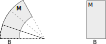
\includegraphics[width=.9\linewidth]{../img/RiemannFibration.png}
\caption{The trivialising map is only a diffeomorphism and not an isometry \label{trivalising-map}}
\end{figure}





\begin{theorem}[Hermann]
\label{thm:Hermann}
If the fibration \(\pi: M \longrightarrow B\) is
of totally geodesic fibres then the diffeomorphisms \(\hat\gamma(0) \longrightarrow
\hat\gamma(1)\) are in fact isometries between fibres and \(M\) is then locally a
Riemannian product of \(B\) and the fibre, now equipped with its unique
metric induced by \(M\).
\end{theorem}

\begin{proof}
We need to prove that the metric on fibres \(\hat g_{(b,f)}\) does not depend on the point
\(f\) of the fibre, i.e. for every basic vector field \(X\), one has \(\mathcal{L}_X\hat g=0\), where by \(\hat g\), we mean the (0,2) symmetric tensor \((Y_1, Y_2)\mapsto \langle
\mathcal{V}Y_1, \mathcal{V}Y_2 \rangle\). Let \(U,V\) be vertical vector fields of \(M\) then
\begin{equation*}
\label{eq:calcul-Hermann}
\begin{split}
X(\hat g(U,V)) &= (\mathcal{L}_X \hat g)(U,V) + \hat g([X,U],V) + \hat g(U, [X,V])\\
       	       &=  \langle \nabla_X U, V \rangle - \langle \nabla_U X, V \rangle + \langle U, \nabla_X V \rangle - \langle U, \nabla_V X \rangle + (\mathcal{L}_X\hat g)(U,V)
\end{split}   
\end{equation*}
Hence \((\mathcal{L}_X \hat g)(U,V) = \langle \nabla_U X, V\rangle + \langle U, \nabla_V
X \rangle = -2 \langle \sff(U,V), X \rangle = 0\). Since the map \(\hat\gamma(0) \mapsto \hat\gamma(1)\) is in the one-parameter group of differomorphism
associate to a basic vector field \(X\), it preserves \(\hat g\).
\end{proof}

\subsubsection{Tension fields and harmonic fibrations.}
\label{sec:org87c8e11}
We will now calculate the tension field of a fibration map \(\pi: M \longrightarrow B\).

\begin{proposition}[]
\label{prop:tension-fibration}
Let \(\pi: M^n \longrightarrow B^{n'}\) be a complete Riemannian fibration then
\begin{enumerate}
\item \(e(\pi) = n/2\).
\item Let \(M_b\) be a fibre of \(\pi\) and \(\iota_{M_b}: M_b \hookrightarrow M\) be
the inclusion. Then \(\tau(\pi) = -\pi_*\tau(\iota_{M_b})\) on \(M_b\).
\end{enumerate}
In particular, \(\pi\) is harmonic if and only if its fibres are minimal submanifolds of
\(M\), i.e. the inclusions \(\iota_{M_b}\) are harmonic.
\end{proposition}
\begin{proof}
\begin{enumerate}
\item is obvious. For 2), note that
\end{enumerate}
\[
\tau(\iota_{M_b}) = -\sum_{\sigma = 1}^{n'}{\rm div\ }(e_\sigma(P))e_\sigma(P)
\]
for any orthonormal frame \(e_\sigma(P)\) of normal vectors of \(M_{\pi(P)}\).
Take \(e_\sigma\) to be \(e_\sigma = {\rm grad\ } \pi^\sigma\) where \(\pi^\sigma\)
is the \(\sigma\)-th component of \(\pi\) in a normal coordinate of \(V\) around \(\pi(P)\). Note that \(e_\sigma\) are actually the horizontal lift of the basis vectors \(\tilde e_\sigma\) of the frame at \(\pi( P)\), and therefore are normal vectors of \(M_P\). 

Meanwhile, one has \(\tau(\pi) = -\Delta \pi^\sigma \tilde e_{\sigma}\) at \(\pi(P)\)
since the Christoffel symbols vanish at \(P\). Comparing the two vector fields, one has
\(\tau(\pi) = -\pi_*\tau(\iota_{M_b})\) at \(P\).
\end{proof}

\begin{exampl}
A complete Riemannian fibration \(\pi: M \longrightarrow B\) with totally geodesic fibres are harmonic.
\end{exampl}

\subsection{Composition of maps}
\label{sec:orgb5b6454}

The following results come from direct computation of the second fundamental form and
tension field of composition of maps between Riemannian manifolds. Again, we use indices
\(i,j,k,\dots\) for \(M\), \(\alpha,\beta,\gamma,\dots\) for \(M'\) and \(a,b,c,\dots\) for \(M''\).

\begin{proposition}
\label{prop:composition-general}
Let \(f: M \longrightarrow M'\) and \(f': M' \longrightarrow M''\) be smooth maps of
Riemannian manifolds, then
\begin{equation}
\label{eq:sff-composition}
\beta(f'\circ f)^a_{ij} = \beta(f)_{ij}^\gamma f'^a_\gamma + \beta(f')_{\alpha\beta}^a f^\alpha_i f^\beta_j
\end{equation}
and
\begin{equation}
\label{eq:tension-field-composition}
\tau(f'\circ f)^a = \tau(f)^\gamma f'^a_\gamma + g^{ij}\beta(f')^a_{\alpha\beta} f^\alpha_i f^\beta_j 
\end{equation}
Therefore,
\begin{center}
\begin{tabular}{lll}
If \(f'\) is & and \(f\)  is & then \(f'\circ f\) is\\
\hline
totally geodesic & totally geodesic & totally geodesic\\
totally geodesic & harmonic & harmonic\\
\end{tabular}
\end{center}
and the inverse of a totally geodesic map is totally geodesic.
\end{proposition}
\begin{proof}
Direct computation.
\end{proof}

\begin{remark}
It is not true in general that the composition of harmonic maps are harmonic.
\end{remark}

\begin{proposition}[composition with immersion]
\label{prop:compo-immersion}
If \(f': M' \longrightarrow M''\) is a Riemannian immersion and \(f: M \longrightarrow
M'\) then 
\begin{enumerate}
\item Energy functionals: \(E(f) = E(f'\circ f)\).
\item Tension fields: \(\tau(f)\) is the projection of \(\tau(f'\circ f)\) to \(M'\).
\end{enumerate}
\end{proposition}
\begin{proof}
\begin{enumerate}
\item One has \(e(f) = \frac{1}{2}\langle g, f^* g' \rangle  = \frac{1}{2}\langle g,
   (f'\circ f)^* g'' \rangle = e(f'\circ f)\).
\item One has \(\tau(f'\circ f)^a  = \tau(f)^a +
   g^{ij}\beta(f')^a_{\alpha\beta} f^\alpha_i f^\beta_j\) by
\eqref{eq:tension-field-composition}. The second term being the restriction of the
tension field of \(M'\) to the image of M, the conclusion follows.
\end{enumerate}
\end{proof}

The following immediate corollary of Proposition \ref{prop:compo-immersion} is a generalization of the fact that a curve is geodesic if and only if it
is perpendicular to its tension field.

\begin{corollary}
A map \(f: M \longrightarrow M'\) is harmonic if and only if \(\tau(f'\circ f) \perp M'\)
\end{corollary}




\begin{proposition}[composition with submersion]
\label{prop:compo-submersion}
Let \(f': M' \longrightarrow M''\) be a Riemannian fibration with totally geodesic
fibres and \(f: M \longrightarrow M'\) then 
\[
\tau(f'\circ f) = f'_*(\tau(f))  
\]
\end{proposition}

\begin{proof}
One can suppose that \(M'\) is a Riemannian product of \(M''\) and its fibre, and
\(f'\) is the projection to \(M''\), since this is true locally and the proposition is
local. Then the conclusion is that the tension field of the projection is the projection
of the tension field, or equivalently the tension field of \(f= f_1\times f_2: M \longrightarrow
M''\times F\) is \(\tau(f) = (\tau f_1,\tau f_2)\). This follows from the explicit
formula of \(\tau(f)\), noting that the Christoffel symbols \(\Gamma^\alpha_{\beta\gamma}\) vanish except when the indice \(\alpha,\beta,\gamma\)
belong to the same tangent space (\(TM''\) or \(TF\)).
\end{proof}

\begin{exampl}
\begin{enumerate}
\item A map \(f: M \longrightarrow M'\times M''\) is harmonic if \(f=(f^1, f^2)\) with \(f^1, f^2\) harmonic.
\item Take \(M''=M\) in Proposition \ref{prop:compo-submersion} and \(f=s: M \longrightarrow M'\) a
section of the fibration \(f'\), one sees that the tension field \(\tau(s)\) is
always vertical.
\end{enumerate}
\end{exampl}

The following corollary is immediate.
\begin{corollary}
\label{cor:compo-with-submersion}
Let \(f': M' \longrightarrow M''\) be a proper Riemannian embedding and \(N\) is a
normal turbular neighborhood of \(M'\) which can be seen as a smooth fiber bundle over
\(M'\). Denote by \(\pi: N \longrightarrow M'\) the projection. Then for all map \(f:
M \longrightarrow N\), \(\pi\circ f\) is harmonic if and only if \(\tau(f)\) is vertical. 
\end{corollary}




\section{Nonlinear heat flow: Global equation and existence of harmonic maps.}
\label{sec:org6190a72}
\subsection{Statement of the main results.}
\label{sec:org69a04d2}

We want to prove in the next part the existence of harmonic map between manifolds \(M\)
and \(M'\) by deforming any map \(f: M
\longrightarrow M'\) using the \(\tau\)-flow, meaning solving the PDE:
\begin{equation}
\label{eq:loc-heat-flow}
\begin{cases}
\frac{d f_t}{d t} = \tau f_t,  & t\in [\alpha,\omega] \\
f_\alpha = f, & 
\end{cases}
\end{equation}
The equation makes sense because both \(\frac{d f_t}{d t}\) and \(\tau f_t\) are
vector fields along \(f_t\). Since this is the gradient-descent equation for \(E\),
the energy of \(f_t\) decreases and we hope, under conditions, to obtain
convergence of \(\{f_t\}\) to a critical point \(f_\infty\) of \(E\), this will prove
that any homotopy class of \(C^\infty(M,M')\) has at least a harmonic map.

It is proved by Eells and Sampson \cite{eells_harmonic_1964} that
\begin{theorem}[Eells-Sampson]
\label{thm:eells-sampson}
Let \(M\) and \(M'\) be compact Riemannian manifolds with \({\rm Riem } (M') \leq 0\) then there exists a harmonic map \(f: M \longrightarrow M'\) in each homotopy class.
\end{theorem}

Several boundary conditions, of Dirichlet, Neumann or mixed type, are also taken into account by Hamilton
\cite{hamilton_harmonic_1975}, as an example, we will state the Dirichlet problem:

\begin{theorem}[Hamilton]
\label{thm:hamilton-bndry-Dirichlet}
Let \(M\) and \(M'\) be compact Riemannian manifolds possibly with boundary. Suppose
that \(M'\) has \({\rm Riem } (M')\leq 0\) and \(\partial M'\) is convex, then any
relative homotopy class of \(C^\infty(M,M')\) has a harmonic element. 
\end{theorem}

About the terminology, \textbf{relative homotopy class} means that we only deform \(f\) among
maps with the same value on \(\partial M\). The \textbf{convexity of \(\partial M'\)} means
that the geodesic at any point in \(\partial M'\) with initial tangent vector paralell
to the boundary does not enter the interior of \(M'\) in short time. This condition can be expressed
using  the Christoffel symbols of \(M'\) at the point in question.

It is easy to see that the convexity of \(\partial M'\) is a necessary condition, as
harmonic maps from \(\mathbb{R}\) are geodesics: Suppose the condition does not hold at
\(x\in \partial M'\), meaning that upto time \(t\) the geodesic flow of \(M'\) initially tangent to
\(\partial M'\) remains in the interior. The geodesic of \(\partial M'\) of length
less than \(t\) with the same initial tangent therefore cannot be deformed into a
geodesic of \(M'\) in relative homotopy class. 

\subsection{Strategy of the proof.}
\label{sec:orgcd4af9e}
In order to have a global frame, we will embed \(M'\) into an Euclidean space \(V\),
but we will not use the Euclidean metric of \(V\). In fact, let \(T\) be a tubular
neighborhood of \(M'\) in \(V\) then if \(T\) is trivial, i.e. if it is diffeomorphic to \(M'\times D\)
where \(D\) is a sufficiently small of dimension being the codimension of \(M'\) in \(V\), and we will equip \(T\) with the product metric of \(M'\times D\). 

If \(T\) is not trivial, use a partition of unity of \(M'\), one can construct a metric on \(T\)
as linear combination of the previously defined metrics on trivialised pieces such that
the involution \(\iota: T \longrightarrow T\) locally given by \((y,d)\mapsto (y,-d)\)
for \(y\in M', d\in D\) is an isometry. As a consequence, \(M'\) is totally geodesic
in \(T\).


Since \(M' \equiv M'\times \{0\}\) is totally geodesic in \(T\), one has for every smooth
function \(f: M \longrightarrow M'\):
\[
 \tau_V (f) = \tau_T(f) = \tau_{M'} (f)
\]

The crucial property we expect for a global equation of \eqref{eq:loc-heat-flow}, is that if
the solution initially is in \(M'\subset V\) then it remains in \(M'\) for all
relevant time \(t>\alpha\). Eells-Sampson \cite{eells_harmonic_1964} did this by using at
the same time 2 different metrics on \(T\), namely the product metric as tubular
neighborhood and the Euclidean metric. I choose to present here the formulation of
Hamilton, which is conceptually simpler with the only drawback being that we need to
establish the uniqueness of solution of \eqref{eq:loc-heat-flow} first.

After having the global equation, we will prove the short time existence of solution by
linearising the equation and using Implicit function theorem. The global formulation and the
proof of short-time existence is independent of the negative curvature hypothesis, which
will only be used later to establish energy estimates and assure the convergence of
long-time solution and the vanishing of its tension field.


\subsection{Global equation and Uniqueness of nonlinear heat equation.}
\label{sec:orgf2de8fe}
\begin{theorem}[Global equation]
\label{thm:global-eq}
If the smooth function \(F_t:\ M\times [\alpha,\beta] \longrightarrow V\) satisfies
\begin{equation}
\label{eq:global-heat}
\frac{d F_t}{dt} = \tau_V(F_t)
\end{equation}
and \(F_t(M\times \{\alpha\}) \subset M'\) then \(F_t(M\times[\alpha,\omega])\subset M'\)
\end{theorem}
\begin{proof}
Let \(\iota\) be the isometry of \(T\) given by \((y,d)\mapsto (y,-d)\) for \((y,d)\in M'\times D \equiv T\) 
and pose \(G_t= \iota F_t\) then \(G_t\) and \(F_t\) coincide initially since \(M'\) is
fixed by \(\iota\). Moreover
\[
\frac{d G_t}{d t} = d\iota . \frac{d F_t}{d t} = d\iota (\tau_V(F_t)) = \tau_V(\iota F_t)=\tau_V(G_t)
\]
We conclude that \(F_t = G_t = \iota F_t\), hence \(F_t\) remains in \(M'\) for all
relevant \(t\), using the following uniqueness of nonlinear heat equation.
\end{proof}

\begin{theorem}[Uniqueness of solution of nonlinear hear equation]
\label{thm:unique-nonlinear-heat}
Let \(f_1,f_2: M\times [\alpha,\omega] \longrightarrow M'\) be \(C^2\)
functions satisfying the non-linear heat equation
\(\frac{d f_i}{d t} = \tau_{M'}(f_i)\), i.e.
\[
 \frac{d f_i}{d t} =-\Delta f^\gamma +g^{ij}\Gamma'^{\gamma}_{\alpha\beta} f^{\alpha}_{i}f^{\beta}_{j}
\]
where \(\Gamma'^\gamma_{\alpha\beta}\) are Christoffel symbols of \(M'\). Suppose that
\(f_1\) and \(f_2\) coincide on \(M\times \{\alpha\}\). Then \(f_1=f_2\) on \(M\times[\alpha,\omega]\).
\end{theorem}

\begin{proof}
It is sufficient to prove the theorem for \(\omega\) very close to \(\alpha\),
therefore by compactness of \(M\), we can suppose that there exists a finite atlas \(M
= \bigcup_i U_i\) with \(f_1 (U_i\times [\alpha,\omega])\) and \(f_2
(U_i,[\alpha,\omega])\) being in the same chart \(V_i\) of \(M'\). We consider the
distance function \(\sigma(a,b) = \frac{1}{2}d_{M'}(a,b)^2\) for \(a,b\in M'\) to
measure the difference between \(f_1\) and \(f_2\) by 
\[
 \rho(x,t) = \sigma(f_1(x,t), f_2(x,t))
\]
The strategy is to prove that there exists \(C>0\) such that \(\frac{d \rho}{d t} \leq
-\Delta + C\rho\), then by \href{elliptic-parabolic.org}{Maximum principle}, one has \(\rho = 0\).

Fix a chart \(U_i\) of \(M\) and the corresponding \(V_i\) of \(M'\), one has by
straightforward calculation:
\begin{align*}
 \frac{d\rho}{d t} &= -\Delta \rho -g^{ij}\left( \frac{\partial^2 \sigma}{\partial
 f_1^\beta \partial f_1^\gamma} - \frac{\partial \sigma}{\partial f_1^\alpha} {\Gamma'}
^{\alpha}_{\beta\gamma}(f_1) \right) {f_1}^\beta_i {f_1}^\gamma_j\\
	        &- g^{ij}\left( \frac{\partial^2 \sigma}{\partial
 f_2^\beta \partial f_2^\gamma} - \frac{\partial \sigma}{\partial f_2^\alpha} {\Gamma'}
^{\alpha}_{\beta\gamma}(f_2) \right) {f_2}^\beta_i {f_2}^\gamma_j - 2g^{ij}\frac{\partial^2 \sigma}{\partial f_1^\beta \partial f_2^\gamma} {f_1}^\beta_i {f_2}^\gamma_j  \\
\end{align*}
where \(g^{ij}\) is the metric on \(M\) and \({\Gamma'}^\alpha_{\beta\gamma}\) are
Christoffel symbols of \(M'\). 


Let \(c\) be a point in the chart \(V_i\) and choose the normal coordinates of \(M'\) at \(c\). Then for \(a,b\in M'\) near \(c\), one has, since \(\sigma(a,b) =
\sigma(b,a)\) and \(\sigma(a,b)=0\) if \(b^\gamma = k a^\gamma\) (the Euclidean
straight line from \(a\) to \(ka\) viewed on \(M'\) is a geodesic):
\[
 \sigma(a,b) = \frac{1}{2}d_{M'}(a,b)^2 = \frac{1}{2}d_E(a,b)^2 +
\lambda_{\beta\gamma,\delta}(a^\beta a^\gamma b^\delta + b^\beta b^\gamma a^\delta)
\]
where \(d_E\) is the Euclidean distance, with \(\lambda_{\beta\gamma,\delta} =
\lambda_{\gamma\beta,\delta}\) and \(\lambda_{\beta\gamma,\delta}
+\lambda_{\gamma\delta,\beta} + \lambda_{\beta\delta,\gamma}= 0\). We then have the
series development of \(\sigma\) at \((0,0)\):
\begin{equation}
\label{eq:dev-sig-unique}
\sigma(a,b) = \frac{1}{2}\delta_{\beta\gamma} (a^\beta - b^\beta)(a^\gamma - b^\gamma) +
\lambda_{\beta\gamma,\delta} (a^\beta a^\gamma b^\delta + b^\beta b^\gamma a^\delta) + O(|a|+|b|)^4
\end{equation}
and the development of its derivatives
\begin{align*}
  \frac{\partial^2 \sigma}{\partial a^\beta \partial b^\gamma}(a,b) &= -\delta_{\beta\gamma} + \lambda_{\beta\delta,\gamma}a^\delta + \lambda_{\gamma\delta,\beta}b^\delta + O(|a|+|b|)^2\\
  \frac{\partial^2 \sigma}{\partial a^\beta \partial a^\gamma}(a,b) &= \delta_{\beta\gamma} + \lambda_{\beta\gamma,\delta}b^\delta + O(|a|+|b|)^2\\
  \frac{\partial^2 \sigma}{\partial b^\beta \partial b^\gamma}(a,b) &= \delta_{\beta\gamma} + \lambda_{\beta\gamma,\delta}a^\delta + O(|a|+|b|)^2\\
   \frac{\partial\sigma}{\partial a^\alpha}(a,b) &= O(|a|+|b|),\quad {\Gamma'}^\alpha_{\beta\gamma}(a) = O(|a|)
\end{align*}
So choose \(c\) to be the midpoint of \(f_1(x,t)\) and \(f_2(x,t)\) and \((f_1(x,t),
f_2(x,t)) = (w,-w)\) in the chart, one has:
\begin{align}
 \frac{d\rho}{d t} &= -\Delta\rho - \left( \delta_{\beta\gamma} -\lambda_{\beta\gamma,\delta}w^\delta + O(|w|^2)  \right) {f_1}^\beta_i {f_1}^\gamma_j g^{ij}   - \left( \delta_{\beta\gamma} + \lambda_{\beta\gamma,\delta} w^\delta + O(|w|^2)\right) {f_2}^\beta_i {f_2}^\gamma_j g^{ij}\\
		   & - 2\left( -\delta_{\beta\gamma} + \lambda_{\beta\delta,\gamma}w^\delta - \lambda_{\gamma\delta,\beta} w^\delta + O(|w|^2)  \right) {f_1}^\beta_i {f_2}^\gamma_j g^{ij} \label{eq:sym-red-beta}\\
		   & = -\Delta \rho - |df_1 -df_2|^2 - w^\delta \lambda_{\beta\gamma,\delta}g^{ij}\left(  {f_2}^\beta_i {f_2}^\gamma_j - {f_1}^\beta_i {f_1}^\gamma_j  \right) \label{eq:first-order-w}
\end{align}
where we made a reduction of the term \eqref{eq:sym-red-beta} by permuting \(\beta\) and
\(\gamma\) to cancel the first order term \(w^\delta\). The last term of \eqref{eq:first-order-w} can be bounded as follows:
\begin{align*}
    \left | w^\delta \lambda_{\beta\gamma,\delta}\left({f_2}^\beta_i {f_2}^\gamma_j -
{f_1}^\beta_i {f_1}^\gamma_j\right) g^{ij} \right| &=   \left | w^\delta \lambda_{\beta\gamma,\delta}\left({f_2}^\beta_i ({f_2}^\gamma_j - {f_1}^\gamma_j) + {f_1}^\gamma_j({f_2}^\beta_i -
{f_1}^\beta_i) \right) g^{ij} \right| \\
	       &\leq 2 |w^\delta \lambda_{\beta\gamma,\delta}| |df_2 -df_1| (|df_1| + |df_2|)\\
	       &\leq |df_1 - df_2|^2 + O(|w|^2)
\end{align*}
where for the last inequality, we use \(2uv \leq u^2 + v^2\) and the fact that \(|df_1|\) and \(|df_2|\) are bounded on \(M\). The estimate \eqref{eq:first-order-w} can be
continued:
\[
 \frac{d \rho}{d t}\leq -\Delta\rho + C(x,t) |w|^2 \leq -\Delta \rho + C \rho
\]
where \(C >0\) is a constant chosen to dominate all \(C(x,t)\) for \(x\in M\) in all
charts and \(t\in [\alpha,\omega]\).
\end{proof}

\begin{remark}
\label{rem:hamilton-alg-rig}
The last proof was modified from \cite{hamilton_harmonic_1975}. The original proof
made the reduction of the first order of \(w\) in \eqref{eq:sym-red-beta} using
the following development of \(\sigma\):
\[
 \sigma = \frac{1}{2}\delta_{\beta\gamma} (a^\beta - b^\beta)(a^\gamma - b^\gamma) +
\lambda_{\beta\gamma,\delta} (a^\beta - b^\beta)(a^\gamma -b^\gamma)(a^\delta + b^\delta) + O(|a|+|b|)^4
\]
which was justified by \(\sigma(a,b) = \sigma(b,a)\) and \(\sigma(a,a)=0\). Algebraically these symmetries of \(\sigma\) are not sufficient to justify the
development, and one can also prove, using \(\sigma(a,ka)= \frac{1}{2}d_E(a,ka)^2\), that if such development
was valid then all \(\lambda_{\beta\gamma,\delta}\) would be zero, and there would be no
third-order term. We made this reduction using the symmetry of \(\frac{\partial^2
\sigma}{\partial f_1^\beta \partial f_2^\gamma} {f_1}^\beta_i {f_2}^\gamma_j\) in \((\beta,\gamma)\) and not just \(\frac{\partial^2
\sigma}{\partial f_1^\beta \partial f_2^\gamma}\) alone.

As a side note, if \(a,b,c\) are on \(\mathbb{S}^2\) with \(d(a,c) = d(b,c) = x \ll 1\)
and the lines from \(a\) and \(b\) to \(c\) are orthogonal at \(c\), then the
geodesic distance \(d(a,b) = \arccos(\cos^2(x)) = x\sqrt{2} - \frac{1}{6\sqrt{2}}x^3 +
O(x^4)\). So \(\sigma(a,b) = \frac{1}{2}d(a,b)^2\) has no third-order term.
\end{remark}

\section{A few energy estimates.}
\label{sec:org08246ad}
\subsection{Estimate of density energies}
\label{sec:org77cb4c6}
We finish this part with a few straightforward computation concerning the \textbf{potential
energy} \(e(f_t) = \frac{1}{2}|\nabla f_t|^2\) and the \textbf{kinetic energy} \(k(f_t) =
\frac{1}{2}|\frac{\partial f_t}{\partial t}|\) of a nonlinear heat flow \(f_t\)
satisfying \eqref{eq:loc-heat-flow}.

\begin{theorem}[Density of Potential energy]
\label{thm:den-pot}
If \(f_t\) satisfies \eqref{eq:loc-heat-flow} then 
\[
 \frac{d e(f_t)}{dt}= -\Delta e(f_t) - |\beta(f_t)|^2 - \left\langle \Ric(M) \nabla_v
f_t,\nabla_v f_t \rangle + \langle \Riem(M') (\nabla_v f_t,\nabla_w f_t)\nabla_v
f_t,\nabla_w f_t \right\rangle
\]
where \(e(f_t)\) is the potential energy density and \(\beta(f_t)\) is the fundamental
form and in the curvature terms, the vectors \(v\) and \(w\) are contracted.

In particular, if  \(\Riem(M') \leq 0\) and \(\Ric(M)\geq -C\) then
\begin{equation}
\label{eq:den-pot-est}
\frac{d e}{dt} \leq -\Delta e + Ce - |\beta(f_t)|^2
\end{equation}
\end{theorem}
\begin{proof}
Apply Lemma \ref{lem:calculs-general} to \(s = d f_t\) and the Riemannian-connected
bundle \((F^* TM'\) over \(M\times [\alpha,\omega]\) where \(F(\cdot,t) = f_t\), the curvature terms cancel
out and it remains to see that
\(\frac{d e(f_t)}{dt}= - \langle df_t, \Delta df_t \rangle\), meaning that \(\tilde \nabla_{\partial t} df_t = -\Delta df_t\). This can be easily
justified:
\[
\tilde \nabla_{\partial t} df_t = \tilde \nabla_{\partial t} \tilde\nabla^M F=  \tilde\nabla^M
\tilde\nabla_{\partial t} F= \tilde\nabla^M\ \tau (f_t) = -D\delta (df_t) = -\Delta df_t
\]
where the last "=" is due to \(D df_t = 0\). Note that \(D\) and \(\delta\)
are the exterior derivative and its adjoint of the bundle \((f_t)^*TM'\) on \(M\),
where \(t\) can be fixed after the third "=" sign.
\end{proof}

\begin{theorem}[Density of Kinetic energy]
\label{thm:den-kin}
If \(f_t\) satisfies \eqref{eq:loc-heat-flow} then 
\[
 \frac{d k(f_t)}{dt}= -\Delta k(f_t) - \left|\nabla \frac{\partial f_t}{\partial t}\right|^2 +
\left\langle \Riem(M') (\nabla_v f_t,\frac{\partial f_t}{\partial t})\nabla_v
f_t,\frac{\partial f_t}{\partial t} \right\rangle
\]
where \(k(f_t)\) is the kinetic energy density and in the curvature terms, the vectors \(v\) is contracted,

In particular, if  \(\Riem(M') \leq 0\) then
\begin{equation}
\label{eq:den-kin-est}
\frac{d k}{dt} \leq -\Delta k  - \left|\nabla \frac{\partial f_t}{\partial t}\right|^2
\end{equation}
\end{theorem}

\begin{proof}
Let \(F:\ I\times M \longrightarrow M'\) be the total function with \(F(t,\cdot)
= f_t\) for \(t\in I =[\alpha,\omega]\) and \(E = F^* TM'\) is a Riemannian-connected bundle on \(I\times M\) with curvature form \(\Theta\), then
\begin{equation}
\label{eq:den-kin-1}
\tilde \nabla_{\partial t} \tilde\nabla_v (dF.v) = \tilde\nabla_v \tilde\nabla_{\partial t} (dF.v) + \Theta(\partial t, v) dF.v
\end{equation}
where \(dF\) is the exterior derivative of \(f_t\) on \(M\). Note that \(\tilde \nabla_v \tilde \nabla_{\partial t} (dF.v) = \tilde \nabla_v (\tilde
\nabla_{\partial t} dF).v = \tilde \nabla_v (\tilde\nabla^M \frac{\partial f_t}{\partial
t}).v\) since \(\tilde\nabla^M \frac{\partial f_t}{\partial t}= \tilde\nabla_{\partial
t}^{I\times M} dF = \tilde\nabla^{I}_{\partial_t}dF\) because
\(\tilde \nabla\) is torsionless on \(M'\). Plugging this in \eqref{eq:den-kin-1} and taking contraction
in \(v\), one has
\begin{equation}
\label{eq:den-kin-2}
 \tilde \nabla_{\partial t}\ \tau(f_t) = -\tilde \Delta \frac{\partial f_t}{\partial t} +
\tr \left( v\mapsto \Theta (\partial t,v) dF.v\right)
\end{equation}
But \(\Theta^\beta_\alpha = R'^\beta_{\alpha\nu\mu} F^\mu_i F^\nu_j dx^i\otimes dx^j\)
where \(R'\) denotes the Riemannian curvature of \(M'\) and the indices \(i,j\) can
be \(0\), with \(x^0 \equiv t\). Hence 
\[
 \Theta (\partial t, v) dF.v = R'^\beta_{\alpha \nu \mu} \frac{\partial f^\mu_t}{\partial
t}\frac{\partial f_t^\nu}{\partial v} \frac{\partial f_t^\alpha}{\partial v} \tilde
e_\beta = \Riem(M')\left(\nabla_v f_t, \frac{\partial f_t}{\partial t}\right)\nabla_v f_t
\]
Plugging in \eqref{eq:den-kin-2} and taking inner product with \(\frac{\partial
f_t}{\partial t}\), one has
\begin{align*}
 \frac{\partial k(f_t)}{\partial t} &= \left\langle \tilde \nabla_{\partial t}\ \tau(f_t),
\frac{\partial f_t}{\partial t} \right \rangle = - \left\langle \tilde \Delta \frac{\partial
f_t}{\partial t}, \frac{\partial f_t}{\partial t} \right\rangle + \left \langle \Riem(M')
(\nabla_v f_t, \frac{\partial f_t}{\partial t}) \nabla_v f_t, \frac{\partial f_t}{\partial
t} \right \rangle  \\
   &= - \Delta \left(\frac{1}{2} \left|\frac{\partial f_t}{\partial t}\right|^2\right) - \left| \tilde \nabla \frac{\partial f_t}{\partial t}\right|^2 + \left \langle \Riem(M')
(\nabla_v f_t, \frac{\partial f_t}{\partial t}) \nabla_v f_t, \frac{\partial f_t}{\partial
t} \right \rangle
\end{align*}
\end{proof}

\subsection{Estimate of total energies}
\label{sec:orgcde4a70}

We will now work with the total energies, in particular the \textbf{total potential energy} \(E(f_t) := \int_M e(f_t)\) and \textbf{total kinetic energy} \(K(f_t) := \int_M k(f_t)\). Since
tension field is the gradient of \(E\), one has:

\begin{theorem}
\label{thm:energy-cons}
If \(f_t: M \longrightarrow  M'\) satisfies \eqref{eq:loc-heat-flow} then
\[
 \frac{d E(f_t)}{dt} = -\int_M \left\langle \tau(f_t), \frac{\partial f_t}{\partial t}
\right \rangle = -\int_M |\tau(f_t)|^2 = -2K(f_t)
\]
and
\[
\frac{d^2 E(f_t)}{dt} = -2\int_M \left \langle \nabla_{\partial t}\frac{\partial
f_t}{\partial t},\tau(f_t)\right \rangle
\]
\end{theorem}

Intergrating Theorem \ref{thm:den-kin} on \(M\), one obtains:

\begin{theorem}
\label{thm:int-den-kin}
If \(f_t\) satisfies \eqref{eq:loc-heat-flow} and \(\Riem(M')\leq 0\) then \(\frac{d
}{dt}K(f_t) \leq 0\). Together with Theorem \ref{thm:energy-cons}, one has
\begin{enumerate}
\item The total potential energy \(E(f_t)\) is \(\geq 0\), decreasing and convex.
\item The total kinetic energy \(K(f_t)\) is \(\geq 0\), decreasing and if \(\omega =
   +\infty\) then \(\lim_{t\to\infty} K(f_t) = 0\).
\end{enumerate}
In particular, \(\int_{M\times \{\tau\}} |\nabla f|^2\) and \(\int_{M\times\{\tau\}} \left|
\frac{\partial f_t}{\partial t} \right|^2\) are bounded above by a constant \(C>0\)
independent of the time \(\tau \in[\alpha,\omega]\).
\end{theorem}
Note that we ruled out the case where \(K(f_t)\) decreases to a strictly positive number
because \(E(f_t)\) is bounded below and \(\frac{d }{d t} E(f_t) = -2K(f_t)\).


Integrating Theorem \ref{thm:den-pot} on \(M\) and use Theorem \ref{thm:int-den-kin}, one has:

\begin{theorem}
\label{thm:int-den-pot}
If \(f_t\) satisfies \eqref{eq:loc-heat-flow} and \(\Riem(M')\leq 0\) and \(\Ric(M)\)
is bounded below then 
\[
\int_M |\beta(f_t)|^2 \leq C
\]
for all time \(t\) where the constant \(C\) only depends on the curvature of \(M, M'\) and the initial total potential and kinetic energy, in particular, \(C\) does not depend on \(t\).
\end{theorem}

This means that \(\|f_t\|_{W^{2,2}(M)}\) is bounded by a constant \(C\) only depending
on the curvatures and initial total energies.


\begin{corollary}[Boundedness in \( W^{2,2}(M) \)]
\label{cor:bound-2-2}
If \(F_t\) satisfies \eqref{eq:global-heat} and \(\Riem(M')\leq 0\) and \(\Ric(M)\)
is bounded below then
\[
\|F_t\|^2_{W^{2,2}(M)} := \int_M | \beta(F_t)|^2 + |\nabla F_t| +|F|^2 \leq C
\]
for all time \(t\) where the constant \(C\) only depends on the curvature of \(M, M'\) and the initial total potential and kinetic energy, in particular, \(C\) does not depend on \(t\).
\end{corollary}

Note that the term \(|F|^2\) is trivially bounded since the image of \(F\) remains in
an Euclidean ball \(B\).


\part{Resolution of nonlinear heat equation on manifold}
\chapter[Short-time existence and regularity for nonlinear heat equation]{Short-time existence and regularity for nonlinear heat equation: Polynomial differential operators and Besov spaces}
\iffalse
\begin{info}
The PDF version of this page can be downloaded by replacing \texttt{html} in the its address by
\texttt{pdf}. 
For example \texttt{/html/sheaf-cohomology.html} should become \texttt{/pdf/sheaf-cohomology.pdf}.
\end{info}
\fi

\begin{definition}
We say that \(P\) is a \textbf{polynomial differential operator of type \((n,k)\)} if \(P\)
is of the form
\[
 P(F) = \sum c_{\alpha_1,\dots, \alpha_\nu} (x, F(x)) D^{\alpha_1} F^{a_1} \dots D^{\alpha_\nu} F^{a_{\nu}}
\]
where the coefficients \(c_{\alpha_1,\dots,\alpha_nu}\) depend smoothly and nonlinearly on \(x\) and \(F\) and \(\alpha_i\in \mathbb{R}^N\) are indices with the weighted norm \(\|\alpha_i\| \leq k\) and \(\sum \|\alpha_i\| \leq n\).
\end{definition}

\begin{exampl}
On \(M\times [\alpha,\omega]\) the tension field \(\tau(F) :=  -\Delta F^\alpha + g^{ij}\Gamma'^\alpha_{\beta\gamma}(F)
F^\beta_i F^\gamma_j\) is a polynomial differential operator of type (2,2). The quadratic
term alone is of type (2,1).
\end{exampl}

\section{A regularity estimate for polynomial differential operator.}
\label{sec:orgde1591a}
Our goal in this part is to prove the following estimate for polynomial differential
operator, in which \(X\) will be \(M\times[\alpha,\omega]\).

\begin{theorem}[Regularity of polynomial differential operator]
\label{thm:reg-poly-diff}
Let \(X\) be a compact Riemannian manifold, \(B\subset \mathbb{R}^N\) is a
large Euclidean ball and \(P\) be a polynomial differential
operator of type \((n,k)\) on \(X\). Suppose that
\begin{equation}
\label{eq:cond:thm:reg-poly-diff}
 r\geq 0,\quad p,q\in (1,\infty),\quad r+k < s, \quad \frac{1}{p}> \frac{r+n}{s} \frac{1}{q}.
\end{equation}
Then for all \(F\in C (X,B) \cap W^{s,q}(X)\), one has \(PF\in W^{r,p}(X)\) and
\[
 \|P F \|_{W^{r,p}} \leq C\left(1 + \|F\|_{W^{s,q}}\right)^{q/p}.
\]
where \(C\) is a constant independent of \(F\).
\end{theorem}

We will prove that the result is \emph{local}, in a sense to be defined. Then we will prove the
local statement using Besov spaces.

\begin{proof}[Proof (reduction of Theorem \ref{thm:reg-poly-diff} to a local statement)]
Let \(\{ \varphi_i: U_i \longrightarrow V_i \}\) be an atlas of \(M\). We denote a point
in \(U_i\) by \(x\) and its coordinates in \(V_i\) by \(\xi\). Let \(\sum \psi_i
= 1\) be a partition of unity subordinated to \(\{U_i\}\) and \(\tilde \psi_i\)
be smooth functions supported in \(U_i\) with \(0\leq \tilde \psi_i \leq 1\) and \(\tilde \psi_i = 1\) in the support of
\(\psi_i\), as in the definition of Sobolev spaces on manifold. We suppose the following local statement is true:
\begin{lemma}[Local statement]
\label{lem:loc-reg-poly-diff}
Let \(P\) be a polynomial differential operator of type \((n,k)\) and coefficients \(c_{\alpha_1,\dots,\alpha_\nu}(x,F)\) are smooth and vanish when \(x\in \mathbb{R}^{\dim X}\) is
outside of a compact. Let \(B\subset \mathbb{R}^N\) be a large Euclidean ball and \(r,p,q,s\) as in \eqref{eq:cond:thm:reg-poly-diff}. Then for all compactly supported  \(F\in C (\mathbb{R}^{\dim X},B)
\cap W^{s,q}(\mathbb{R}^{\dim X})\), one has
\[
 \|P F \|_{W^{r,p}} \leq C\left(1 + \|F\|_{W^{s,q}}\right)^{q/p}
\]
where the constant \(C\) depends only on \(B\) and the support of \(F\), and not on \(F\).
\end{lemma}
One has
\[
\| PF \|_{W^{r,p}} := \sum_i \|\psi_i P F\|_{W^{r,p}}
\]
where viewed in the chart \(U_i\), each \(\psi_i(x) PF(x)\) is \(\sum_\alpha\psi_i(\xi). c_\alpha
(\xi,g_i). D^\alpha g_i\) where \(g_i = f_i\circ \varphi_i^{-1}\) is \(f_i\) viewed in
the chart. Since \(\tilde \psi_i = 1\) in the support of \(\psi_i\), one has
\[
 \psi_i(\xi). c_\alpha (\xi,g_i). D^\alpha g_i = \psi_i(\xi). c_\alpha(\xi,\tilde \psi_i g_i) D^\alpha
(\tilde\psi_i g_i)
\]
hence by the local statement:
\[
\| \psi_i(\xi). c_\alpha (\xi,g_i). D^\alpha g_i \|_{W^{r,p}} \leq C \left( 1 + 
\|\tilde \psi_i g_i\|_{W^{s,q}} \right)^{q/p} \leq C \left( 1 + \|F \|_{W^{s,q}}\right)^{q/p}.
\]
Therefore \(\|PF\|_{W^{r,p}} \leq m C \left( 1 + \|F \|_{W^{s,q}}\right)^{q/p}\) where
\(m\) is the number of charts we used to cover \(M\).
\end{proof}
\begin{remark}
The use of partition of unity in the last proof is to decompose \(PF = \sum \psi_i PF\)
and not \(F = \psi_i F\) since we no longer have linearity of the operator \(P\) in \(F\).
\end{remark}

\section{Review of Besov spaces \(B^{s,p}\).}
\label{sec:org9828763}
In this part, \(X = \mathbb{R}^n\) coordinated by \((x_1,\dots,x_n)\) with weight \((\sigma_1,\dots,\sigma_n)\). We define
\[
 T_j^v f(x_1,\dots,x_n) := f(x_1,\dots, x_j +v,\dots, x_n),\quad \Delta^v_j := T^v_j - {\rm Id}
\]
for \(f\in \mathcal{S}(X)\).

For the notation, we will denote the Besov spaces by \(B^{s,p}\) with \(s\in \mathbb{R}_{>0}\setminus
\mathbb{Z}\) and \(p\in (1,\infty)\) so that they look similar to Sobolev space \(W^{s,p}\). In \href{https://en.wikipedia.org/wiki/Besov\_space}{a more standard notation}, our spaces \(B^{s,p}\) are denoted by \(B^{s}_{p,p}\)

\begin{definition}
We define \(B^{s,p}\) as the completion of \(\mathcal{S}(X)\) under the norm
\[
\|f\|_{B^{s,p}} := \sum_{\|\gamma\| < s} \|D^\gamma f\|_{L^p} +
\sum_{ s- \frac{\sigma}{\sigma_j} < \|\gamma\| < s}\sup_{v} \frac{\|\Delta^v_j D^\gamma
f\|_{L^p}}{|v|^{(s - \|\gamma\|) \sigma_j/\sigma}}
\]
\end{definition}

We cite here some well-known facts
\begin{enumerate}
\item While Sobolev spaces with non-integral regularity are complex interpolation of integral
ones, Besov spaces are their real interpolation.
\item Besov spaces \(B^{s,p}(X)\) are reflexive Banach spaces with their dual spaces being
\(B^{-s,p'}(X)\) where \(\frac{1}{p} + \frac{1}{p'}=1\).
\end{enumerate}

\begin{theorem}
\label{thm:besov-sobolev}
If \(r < s\) then
\[
 W^{s,p}(X) \subset B^{s,p}(X) \subset W^{r,p}(X).
\]
\end{theorem}

\begin{theorem}[Multiplication]
\label{thm:estimate-product}
For \(f,g\in \mathcal{S}(X)\) and \(\begin{cases}
0<\alpha <1, \tilde p \leq p,\tilde q \leq q,\tilde r\leq r \\
\frac{1}{p} + \frac{1}{q} = \frac{1}{r}, \frac{1}{\tilde p} + \frac{1}{q} = \frac{1}{p} +
\frac{1}{\tilde q} = \frac{1}{\tilde r}				      
				       \end{cases}\),  one has
\begin{align}
\|fg\|_{B^{\alpha,\tilde r}} &\leq C \left( \|f\|_{B^{\alpha,\tilde p}}\|g\|_{L^q} + \|f\|_{L^p}\|g\|_{B^{\alpha,\tilde q}} \right) \label{eq:estimate-product-1} \\
\|fg\|_{L^r} &\leq \|f\|_{L^p}\|g\|_{L^q} \label{eq:estimate-product-2}
\end{align}
Therefore by density \eqref{eq:estimate-product-1} is true for all \(f\in L^p\cap
B^{\alpha,\tilde p}, g\in L^q\cap B^{\alpha,\tilde q}\) and \eqref{eq:estimate-product-2}
is true for all \(f\in L^p, g\in L^q\).
\end{theorem}

The reason for which we use the Besov norm is the following estimate:
\begin{theorem}[Composition]
\label{thm:compo-besov}
Let \(\Gamma(x,y)\) be a continuous, nonlinear function of variables \(x\in
\mathbb{R}^n, y\in \mathbb{R}^N\). Suppose that \(\Gamma\) vanishes for all \(x\)
outside of a compact in \(\mathbb{R}^n\) and \(\Gamma\) is \(C\)-Lipschitz in \(y\), and define
\[
\Gamma f:= \left( x\longmapsto \Gamma(x,f(x)) \right).
\]
Then 
\[ 
\|\Gamma f\| \leq C\left( 1+ \|f\|_{B^{\alpha,p}}\right)
\]
\end{theorem}


\section{Proof of the local estimate.}
\label{sec:org63db1f4}
Since \(B^{r+\epsilon,p}(X)\subset W^{r,p}(X)\), by increasing \(r\) a bit, we can
suppose that \(r\not\in \mathbb{Z}\) and replace the \(W^{r,p}\) norm in the statement
by the \(B^{r,p}\) norm, that is to estimate:
\[
 \|PF\|_{B^{r,p}} = \sum_{\|\gamma\| < r} \| D^\gamma(PF)\|_{L^p} + \sum_{
r-\sigma/\sigma_j< \|\gamma\| < r} \frac{\| \Delta^v_j D^\gamma (PF)\|_{L^p}}{|v|^{(r-\|\gamma\|)\sigma_j/\sigma}}
\]
where 
\begin{equation}
\label{eq:term-small}
 D^\gamma (PF) = \sum c_{\beta_1,\dots,\beta_\mu}(x,F) D^{\beta_1} f^{b_1}\dots D^{\beta_\mu}f^{b_\mu}
\end{equation}
with \(\max \|\beta_i\| \leq k +\|\gamma\|\) and \(\sum \|\beta_i\|\leq n + \|\gamma\|\).

Using \(\Delta^v_j (fg) = \Delta^v_j f\ T^v_j g + f \Delta^v_j g\), one can see that \(\Delta^v_j D^\gamma (PF)\) is a sum of terms of 2 types:
\begin{equation}
\label{eq:term-c}
\Delta^v_j c_{\beta_1,\dots,\beta_\mu}\ T^v_j(D^{\beta_1}f^{b_1})\dots T^v_j (D^{\beta_\mu}
f^{b_\mu})
\end{equation}
and
\begin{equation}
\label{eq:term-f}
 c_{\beta_1,\dots,\beta_\mu}\ D^{\beta_1}f^{b_1}\ \dots \ D^{\beta_{i-1}}f^{b_{i-1}}\ \Delta^v_j
(D^{\beta_i} f^{b_i})\ T^v_j(D^{\beta_{i+1}} f^{b_{i+1}})\ \dots\ T^v_j(D^{\beta_\mu} f^{b_\mu})
\end{equation}

Our strategy is to use Theorem \ref{thm:estimate-product} to estimate the terms
\eqref{eq:term-small}, \eqref{eq:term-c} and \eqref{eq:term-f} as follows, where we denote \(\|g\|_p:= \|g\|_{L^p}\)
\begin{equation}
\label{eq:est-term-small}
\left\| c_{\beta_1,\dots,\beta_\mu}(x,F)\ D^{\beta_1} f^{b_1}\dots D^{\beta_\mu}f^{b_\mu} \right\|_{p} \leq \|c_{\beta_1,\dots,\beta_\mu} \|_{\infty}.\|D^{\beta_1} f^{b_1}\|_{p_1}\dots \|D^{\beta_\mu} f^{b_\mu}\|_{p_\mu}
\end{equation}

\begin{equation}
\label{eq:est-term-c}
\left\| \Delta^v_j c_{\beta_1,\dots,\beta_\mu}\ T^v_j(D^{\beta_1}f^{b_1})\dots T^v_j (D^{\beta_\mu}
f^{b_\mu})  \right\|_p \leq \|\Delta^v_j c_{\beta_1,\dots,\beta_\mu}\|_{\tilde p_0}. \| D^{\beta_1} f^{b_1} \|_{p_1}\dots \|D^{\beta_\mu} f^{b_\mu}\|_{p_\mu}
\end{equation}

\begin{multline}
\label{eq:est-term-f}
\left\| c_{\beta_1,\dots,\beta_\mu}\ D^{\beta_1}f^{b_1}\ \dots \ D^{\beta_{i-1}}f^{b_{i-1}}\ \Delta^v_j
(D^{\beta_i} f^{b_i})\ T^v_j(D^{\beta_{i+1}} f^{b_{i+1}})\ \dots\ T^v_j(D^{\beta_\mu} f^{b_\mu}) \right\|_p \leq  \\ \|c_{\beta_1,\dots,\beta_\mu}\|_\infty. \| D^{\beta_1}f^{b_1} \|_{p_1}\dots \| D^{\beta_{i-1}}f^{b_{i-1}}\|_{p_{i-1}}. \|\Delta^v_j
(D^{\beta_i} f^{b_i}) \|_{\tilde p_i}. \| D^{\beta_{i+1}} f^{b_{i+1}} \|_{p_{i+1}}\dots \|D^{\beta_\mu} f^{b_\mu} \|_{p_\mu}
\end{multline}

Then continue by bounding the \(\Delta^v_j\) terms:
\begin{equation}
\label{eq:est-del-c}
\|\Delta^v_j c_{\beta_1,\dots,\beta_\mu}\|_{\tilde p_0} \leq |v|^{\theta \sigma_j/\sigma} C (1+ \|F\|_{B^{\theta,\tilde p_0}}) \leq |v|^{\theta \sigma_j/\sigma} C (1+ \|F\|_{W^{\theta,\tilde p_0}})
\end{equation}
using Theorem \ref{thm:compo-besov}, where \(C\) is the Lipschitz constant of \(c_{\beta_1,\dots,\beta_\mu}(x,F)\) in \(F\), which exists because \(c_{\beta_1,\dots,\beta_\mu}\) is smooth and \(F\) always
remains in a large Euclidean ball \(B\). The next \(\Delta^v_j\) term to bound is,
using Theorem \ref{thm:besov-sobolev}:
\begin{equation}
\label{eq:est-del-f}
\|\Delta^v_j (D^{\beta_i} f^{b_i}) \|_{\tilde p_i}\leq |v|^{\theta \sigma_j/\sigma} \|f^{b_i}\|_{B^{\|\beta_i\| +\theta, \tilde p_i}} \leq |v|^{\theta \sigma_j/\sigma} \|f^{b_i}\|_{W^{\|\beta_i\| +\theta, \tilde p_i}}
\end{equation}

And finally plugging \eqref{eq:est-del-c} and \eqref{eq:est-del-f} in \eqref{eq:est-term-c} and
\eqref{eq:est-term-f}, and noting that \(\|c_{\beta_1,\dots,\beta_\mu} \|_{\infty}\) in
\eqref{eq:est-term-small} is bounded by a constant, it remains to estimate \(\| f^{b_i}
\|_{W^{\|\beta_i\|, p_i}}\), \(\| f^{b_i}
\|_{W^{\|\beta_i\| + \theta, \tilde p_i}}\) and \(\|F\|_{W^{\theta, \tilde p_0}}\) in
term of \(\|F\|_{W^{s,q}}\), for which we will use the following consequence of Interpolation
inequality.

\begin{lemma}
\label{lem:loc-est-reg}
Let \(0\leq r\leq s\) and \(p,q\in (1, \infty)\) such that \(0 <
\frac{1}{p} - \frac{r}{s}\frac{1}{q} < 1-\frac{r}{s}\). Then for all compactly supported \(F\in C(X, B)\cap W^{s,q}\) where \(B\subset \mathbb{R}^N\) is a large Euclidean ball, one has
\[
 \|F\|_{W^{r,p}} \leq C \|F\|^{1-r/s}_\infty \|F\|^{r/s}_{W^{s,q}}\leq C' \|F\|^{r/s}_{W^{s,q}}
\]
where \(C,C'\) depend only on \(B\) and the support of \(F\), but not \(F\).
\end{lemma}

\begin{proof}
Since \(F\) is bounded, \(f^\alpha\in W^{s,q} \cap W^{0,v}\) for all \(v > 1\). By
Interpolation inequality
\[
 \|f^\alpha\|_{W^{r,p}} \leq 2 \|f^\alpha\|^{r/s}_{W^{s,q}} \|f^\alpha\|^{1-r/s}_{W^{0,v}}
\]
then choose \(v\) with \((1 - \frac{r}{s})\frac{1}{v} = \frac{1}{p} -
\frac{r}{s}\frac{1}{q}\).
\end{proof}

To apply Lemma \ref{lem:loc-est-reg}, we have to choose \(p_i,\tilde p_i, \tilde p_0,\theta\) such that 
\begin{cases}
0< \frac{1}{p_i} - \frac{\|\beta_i\|}{s} \frac{1}{q} < 1 - \frac{\|\beta_i\|}{s},   \\
0< \frac{1}{\tilde p_i} - \frac{\|\beta_i +\theta\|}{s}\frac{1}{q} < 1 - \frac{\|\beta_i +\theta\|}{s} \\
0< \frac{1}{\tilde p_0} - \frac{\theta}{s}\frac{1}{q} < 1- \frac{\theta}{s}
\end{cases}
We choose \(\frac{1}{p_i}\) just a bit bigger than \(\frac{\|\beta_i\|}{s}\frac{1}{q}\),
\(\frac{1}{\tilde p_i}\) just a bit bigger than \(\frac{\|\beta_i
+\theta\|}{s}\frac{1}{q}\) and \(\frac{1}{\tilde p_0}\) just a bit bigger than
\(\frac{\theta}{s}\frac{1}{q}\). We will now come back to justify the estimates
\eqref{eq:est-term-small}, \eqref{eq:est-term-c}, \eqref{eq:est-term-f}. Since \(F\) is
bounded in \(B\) and compactly supported in an open set \(V\), we see that \(\|f^\alpha\|_p \leq
C(B,V) \|f^\alpha\|_q\) if \(p\leq q\). Therefore,
\begin{enumerate}
\item For \eqref{eq:est-term-small}, it is sufficient to have
\[
    \frac{1}{p} \geq \frac{1}{p_1}+\dots + \frac{1}{p_\mu} 
   \]
 which is true because the RHS is is a bit bigger than \(\frac{1}{qs}\sum \|\beta_i\|
   \leq \frac{n + \|\gamma\|}{qs} < \frac{n+r}{qs} < \frac{1}{p}\).
\item For \eqref{eq:est-term-c}, it is sufficient to have
\[
    \frac{1}{p} \geq \frac{1}{\tilde p_0} + \frac{1}{p_1}+\dots + \frac{1}{p_\mu} 
   \]
 where the RHS is is a bit bigger than \(\frac{\theta}{s}\frac{1}{q}+ \frac{1}{qs}\sum \|\beta_i\|
   \leq \frac{n + \|\gamma\| + \theta}{qs}\).
\item For \eqref{eq:est-term-f}, it is sufficient to have
\[
    \frac{1}{p} \geq  \frac{1}{p_1}+\dots + \frac{1}{\tilde p_i} + \dots + \frac{1}{p_\mu} 
   \]
where the RHS is is a bit bigger than \(\frac{\theta}{s}\frac{1}{q}+ \frac{1}{qs}\sum \|\beta_i\|
   \leq \frac{n + \|\gamma\| + \theta}{qs}\).
\end{enumerate}

It is sufficient then to take \(\theta = r- \|\gamma\|\). Now the estimates
\eqref{eq:est-term-small}, \eqref{eq:est-term-c}, \eqref{eq:est-term-f} can be continued as
\begin{align}
  RHS \eqref{eq:est-term-small} &\leq \prod_i \|f^{b_i}\|^{\|\beta_i\|/s}_{W^{s,q}} \leq \|F\|_{W^{s,q}}^{\frac{n+\|\gamma\|}{s}} \leq \|F\|_{W^{s,q}}^{q/p}\label{eq:fin-del-small}\\
  RHS \eqref{eq:est-term-c} &\leq |v|^{\theta\sigma_j/\sigma}\left( 1 + \|F\|_{W^{s,q}}^{\theta/s} \right)\prod_i \|f^{b_i}\|^{\|\beta_i\|/s}_{W^{s,q}}\leq |v|^{\theta\sigma_j/\sigma}\left( 1 + \|F\|_{W^{s,q}}^{\theta/s} \right)\|F\|_{W^{s,q}}^{q/p} \label{eq:fin-del-c}\\
  RHS \eqref{eq:est-term-f} &\leq |v|^{\theta\sigma_j/\sigma}\left( 1 + \|f^{b_i}\|_{W^{s,q}}^{\frac{\|\beta_i\| +\theta}{s}} \right)\prod_{u\ne i} \|f^{b_u}\|^{\|\beta_u\|/s}_{W^{s,q}}\leq |v|^{\theta\sigma_j/\sigma}\left( 1 + \|F\|_{W^{s,q}}^{\frac{\|\beta_i\| +\theta}{s}} \right)\|F\|_{W^{s,q}}^{q/p} \label{eq:fin-del-f}
\end{align}
While \eqref{eq:fin-del-small} gives \(\|D^\gamma (PF)\|_p \leq C \|F\|_{W^{s,q}}^{q/p}\),
the last two \eqref{eq:fin-del-c} and \eqref{eq:fin-del-f} give
\[
 \sum_{ s- \frac{\sigma}{\sigma_j} < \|\gamma\| < s}\sup_{v} \frac{\|\Delta^v_j D^\gamma (PF) \|_p}{|v|^{(r-\|\gamma\|)\sigma_j/\sigma}} \leq C \left(
1 + \|F\|^{(n+r)/s}_{W^{q,s}}\right)
\]
We proved the local statement Lemma \ref{lem:loc-reg-poly-diff}.


\chapter[Global existence for nonlinear heat equation]{Global existence for nonlinear heat equation and harmonic maps between Riemannian manifolds}
\iffalse
\begin{info}
The PDF version of this page can be downloaded by replacing \texttt{html} in the its address by
\texttt{pdf}. 
For example \texttt{/html/sheaf-cohomology.html} should become \texttt{/pdf/sheaf-cohomology.pdf}.
\end{info}
\fi

Let \(M\) be a compact Riemannian manifold. We want to solve the following nonlinear
heat equation where \(F: M \longrightarrow M'\subset
B\subset V = \mathbb{R}^N\):
\[
 \frac{d F_t}{d t} = -\Delta F_t + \Gamma(F_t) (\nabla F_t)^2
\]
We have proved that the solution \href{polynomial-besov.org}{exists in short-time and is smooth whenever it exists}. We will now establish long-time existence using continuity
method: we will show that if the solution exists on \([\alpha,\omega_n]\) where
\(\omega_n\) is an increasing sequence to \(\omega\), then the solution exists on \([\alpha,\omega]\). We then apply short-time existence to gain a small open interval where
solution still exists. We then conclude that the solution exists globally on \([\alpha,+\infty)\) since this interval is connected.

The crucial step to prove that the solution can be extended on \([\alpha,\omega]\) is to
uniformly bound all of its derivatives in time of evolution \([\alpha,\omega)\). These
estimates will also be useful to justify the convergence of \(F_t\) in \(C^\infty(M)\) to a smooth function \(F_\infty\) which will eventually be a harmonic map
from \(M\) to \(M'\).

Recall that we \href{harmonic-maps.org}{proved} in Corollary \ref{cor:bound-2-2}, under the hypothesis of negative curvature, the boundedness of \(\|F_t\|_{W^{2,2}(M)}\) by a constant \(C\) depending only on curvatures of \(M, M'\) and
the initial total energies. Since \(\frac{dF_t}{dt }\) relates to spatial derivatives of
\(F\) by the nonlinear heat equation, it is easy to see that \(\|F_t\|_{W^{2,2}(M\times[\tau,\tau +\delta])}\) is bounded by a constant independent of
\(\tau\). We will denote \(W^{k,p}(M\times [\beta,\gamma])\) by \(W^{k,p}([\beta,\gamma])\).

\begin{theorem}[\(W^{2,2}\)-boundedness]
\label{thm:bound-2-2}
Suppose \(\Riem(M') \leq 0\). There exists a constant \(C\) depending only on \(\delta\), the metrics and initial
total energies such that
\[
 \|F\|_{W^{2,2}(\tau,\tau+\delta)}\leq C\quad\text{for all } \alpha \leq \tau <\omega-\delta.
\]
\end{theorem}
\begin{proof}
Since 
\[ \|F\|^2_{W^{2,2}([\tau,\tau+\delta])} \leq \int_\tau^{\tau+\delta}
\|F_t\|^2_{W^{2,2}(M)} dt + 2\int_\tau^{\tau+\delta} \left\| \Delta F_t
\right\|^2_{L^2}dt + 2\int_\tau^{\tau+\delta} \left\| \Gamma(F_t)(\nabla F_t)^2
\right\|^2_{L^2}dt
\]
The first term and the second term are bounded by \(C^2\delta\), the third one, since \(\Gamma(F_t)\) is bounded, by \(C^2\delta\) where \(C\) is a constant only depending on
the metrics and initial total energies.
\end{proof}

The estimates of higher derivatives of \(F\) will be established in the same strategy as
the bootstrap: first in \(W^{2,p}\) for all \(p\) then in \(W^{k,p}\) for all \(k,p\), then in \(C^\infty\).

\section{Estimate of higher derivatives.}
\label{sec:org50e3df5}

\begin{lemma}[\( W^{2,p} \)-boundedness]
\label{lem:bound-2-p}
Suppose \(\Riem(M') \leq 0\). For all \(p \in (1,+\infty)\), there exists a constant \(C>0\) depending only on \(\delta\), \(p\), the metrics and initial energies such that for all \(\alpha +\delta \leq \tau \leq \omega-\delta\):
\[
\|F\|_{W^{2,p}([\tau,\tau+\delta])}\leq C
\]
\end{lemma}

\begin{proof}
Applying Gårding Inequality to the parabolic equation \(AF = \Gamma(F) (\nabla F)^2\)
where \(A:= \frac{\partial}{\partial t} + \Delta\) is the heat operator, one has
\[
 \|F\|_{W^{2,p}([\tau,\tau+\delta])} \leq C\left( \|\Gamma(F)(\nabla F)^2\|_{L^p([\tau
 -\frac{\delta}{3},\tau +\delta ])} + \|F\|_{W^{2,2}([\tau-\frac{\delta}{3},\tau +\delta])}  \right)
\]
The second term of RHS is already bounded by applying Theorem \ref{thm:bound-2-2} to \(\frac{4\delta}{3}\). For the first term:
\[
\left\| \Gamma(F) (\nabla F)^2\right\|_{L^p([\tau-\frac{\delta}{3},\tau+\delta])} \leq
C(M') \| |\nabla F|^2 \|_{L^p([\tau-\frac{\delta}{3}, \tau+\delta])} = C(M') \| e(F)
\|_{L^p([\tau - \frac{\delta}{3},\tau+\delta])}.
\]


Recall that by Theorem \ref{thm:den-pot}, the \href{harmonic-maps.org}{potential density} satisfies \(\frac{de}{dt} +\Delta e -Ce \leq 0\) for
certain constant \(C\) depending only on the metric of \(M\). By \href{elliptic-parabolic.org}{Maximum principle}
(Theorem \ref{thm:max-princ-d}), one has \(e \leq \psi_\tau\) where \(\psi_\tau\) is
the solution of

\begin{cases}
\frac{d}{dt}\psi_\tau + \Delta\psi_\tau -C\psi_\tau = 0  \\
\restr{\psi_\tau}{\tau - \frac{\delta}{2}} = \restr{e}{\tau - \frac{\delta}{2}}
\end{cases}

We apply Gårding Inequality again for \(\psi_\tau\) and obtain
\begin{equation}
\label{eq:lem:bound-2-p:2}
 \| e(F) \|_{L^p([\tau - \frac{\delta}{3},\tau+\delta])} \leq \|\psi_\tau\|_{L^p([\tau-
\frac{\delta}{3},\tau+\delta])} \leq C \|\psi_\tau\|_{L^1([\tau-
\frac{\delta}{2},\tau+\delta])}.
\end{equation}


Now apply \(L^1\)-\href{elliptic-parabolic.org}{Comparison Theorem} \ref{thm:1-comparison-d} to \(\psi_\tau\), one has
\begin{equation}
\label{eq:lem:bound-2-p:3}
\|\psi_\tau\|_{L^1([\tau-
\frac{\delta}{2},\tau+\delta])} \leq \int_0^{3\delta/2} \|\restr{\psi_\tau}{\tau-\frac{\delta}{2}}\|_{L^1}e^{Bt}dt \leq \int_0^{3\delta/2}e^{Bt}dt.  \|\restr{e}{\tau-\frac{\delta}{2}}\|_{L^1}\leq C.
\end{equation}
The lemma follows from \eqref{eq:lem:bound-2-p:2} and \eqref{eq:lem:bound-2-p:3}.
\end{proof}

We can now estimate higher order derivatives.

\begin{theorem}[\( W^{k,p} \)-boundedness]
\label{thm:bound-k-p}
Suppose \(\Riem(M') \leq 0\). For all \(p\in (1,+\infty)\) and \(k<+\infty\), there exists \(C\) depending only on
\(k\), \(p\), the metrics and initial energies such that
\[
\|F\|_{W^{k,p}([\tau, \tau+\delta])} \leq C
\]
for all \(\alpha +\delta \leq\tau\leq\omega-\delta\).
\end{theorem}
\begin{proof}
Applying Gårding Inequality to the equation \(\frac{dF}{dt} + \Delta F_t =
\Gamma(F)(\nabla F)^2\) then Regularity estimate for the quadratic term (Theorem \ref{thm:reg-quad}), one has for \(\epsilon \ll \delta\):
\begin{align*}
 \|F\|_{W^{k,p}([\tau,\tau+\delta])} &\leq C_\epsilon \left(
\|F\|_{W^{2,p}([\tau-\epsilon,\tau+\delta])} + \|\Gamma(F)(\nabla F)^2\|_{W^{k-2,p}([\tau-\epsilon,\tau+\delta])}\right)  \\
					   &\leq C_\epsilon\left(1 + C\left(1+\|F\|_{W^{s,q}([\tau-\epsilon,\tau+\delta])}\right)^{q/p}\right)
\end{align*}
as long as \(k-1 < s\) and \(\frac{1}{p} > \frac{k}{s}.\frac{1}{q}\). Therefore if \(\|F\|_{W^{s,q}([\tau,\tau+\delta])}\leq C(\delta,s,q)\) for all \(\beta\leq
\tau\leq\omega-\delta\) and \(q\in (1,+\infty)\), we just proved that
\[
 \|F\|_{W^{k,p}([\tau,\tau+\delta])} \leq C({\epsilon}, k,p)
\]
for all 
\begin{cases}
\beta + \epsilon \leq \tau \leq \omega-\delta \\
k < s+1, p \in(1,+\infty)
\end{cases}
since \(\|F\|_{W^{s,q}([\tau-\epsilon,\tau+\delta])} \leq 2C(\delta,s,q)\).

One can then conclude by induction on \(k\), with step \(\frac{1}{2}\), starting with
\(k=2\) and \(\epsilon=\frac{\delta}{2}\) divided by 2 after each induction step.
\end{proof}


\section{Global existence for nonlinear heat equation.}
\label{sec:orga0359a0}

\begin{theorem}[Global existence]
\label{thm:global-heat-existence}
Suppose \(\Riem(M') \leq 0\). The solution of nonlinear heat equation
\begin{equation}
\label{eq:thm:global-heat}
 \frac{dF}{dt} = -\Delta F +\Gamma(F) (\nabla F)^2
\end{equation}
with smooth initial condition exists globally for all time \(t >\alpha\).
\end{theorem}

\begin{proof}
Let \(F_n\) be a sequence of solution of \eqref{eq:thm:global-heat} on \([\alpha,\omega_n]\) with \(\omega_n\) increasing to \(\omega\) then they coincide by
uniqueness of the solution. As discussed in the beginning of this part, it is
sufficient to prove that the solution extends to \([\alpha,\omega]\). Let \(F\) be the
solution on \([\alpha,\omega)\) such that \(\restr{F}{[\alpha,\omega_n]} = F_n\), then
by Theorem \ref{thm:bound-k-p}, for all \(\tau \in [\alpha,\omega-\delta)\):
\[
 \| D^u_t D^v_x F \|_{L^\infty(M\times[\tau,\tau+\delta])} \leq C_{\rm Sobolev} \| D^u_t D^v_x F
\|_{W^{k,p}(M\times[\tau,\tau+\delta])} \leq C_{\rm Sobolev} . C(k,p,\delta)
\]
where, if we choose \(k\) sufficiently large, \(C_{\rm Sobolev}\) is the constant of Sobolev imbedding \(W^{k,p}(M\times[0,\delta]) \hookrightarrow C(M\times[0,\delta])\) and \(C(k,p,\delta)\)
is the constant provided by Theorem \ref{thm:bound-k-p}. 

So all partial derivatives of \(F\) are uniformly bounded on \([\alpha,\omega)\). This proves that \(F\) extends
to a solution on \([\alpha,\omega]\). In fact \(\restr{F}{\tau}:=\restr{F}{M\times\{\tau\}}\) converges
in \(C^\infty(M)\) as \(\tau\to \omega\), since 
\[ \|D^\alpha \restr{F}{\tau} -
D^\alpha\restr{F}{\tau'}\|_{L^\infty} \leq \max_{\|\beta\| =
\|\alpha\|+1}\|D^{\beta}F\|_{L^\infty}|\tau-\tau'|. 
\]
\end{proof}

We have just proved the first part of the following theorem.

\begin{theorem}[Eells-Sampson]
\label{thm:final}
\begin{enumerate}
\item Let \(M, M'\) be compact Riemannian manifolds with \(\Riem(M') \leq 0\). Then for
every smooth map \(f_0:\ M \longrightarrow M'\subset B\subset \mathbb{R}^N\), the
nonlinear heat equation
\begin{equation*}
\begin{cases}
\frac{df_t}{dt} = \tau(f_t),  & \text{for all $t\geq 0$} \\
\restr{f}{t=0} = f_0,
\end{cases}      
\end{equation*}
admits a globally defined smooth solution \(f_t\). Moreover, all derivatives \(D^\alpha
   f_t\) remain bounded as \(t\to +\infty\).
\item For a suitable sequence \(\{t_n\}\) increasing to \(+\infty\) the sequence \(\{f_{t_n}\}\) converges in \(C^\infty(M)\) to a function \(f_\infty\) with \(\tau(f_\infty)=0\). Therefore any map \(f_0:\ M \longrightarrow M'\) is homotopic to a harmonic map.
\end{enumerate}
\end{theorem}
\begin{proof}
For any sequence \(\{t_n\}\), one can extract from \(\{f_{t_n}\}\), since their derivatives are
uniformly bounded, a subsequence \(\{f_{t_{n_i}}\}\) converging in \(C^k(M,
\mathbb{R}^N)\). By a diagonal argument, one can extract from any sequence \(\{f_{t_n}\}\) a subsequence converging in \(C^\infty(M, \mathbb{R}^N)\) to \(f_\infty\). Abusively denote this subsequence by \(\{f_{t_n}\}\), by Theorem \ref{thm:den-kin}
\[
 \lim_{n\to\infty} K(f_{t_n}) = \lim_{n\to\infty} \int_M |\tau(f_{t_n})|^2 = 0
\]
Therefore \(\tau(f_{t_n}) \to 0\) in \(L^2(M)^{\oplus N}\). But also \(\tau(f_{t_n})
\to \tau(f_\infty)\) in \(C^\infty(M, \mathbb{R}^N)\), one has \(\tau(f_\infty)=0\).
\end{proof}


\part{Existence using Morse-Palais theory}
\chapter{Minimal immersions of $\mathbb{S}^2$}
\input{minimal-immersion-S2.tex}

\part{Appendices: Resolution of linear equations on manifold}

\chapter{Interpolation theory and Sobolev spaces on compact manifolds }
\input{interpolation-sobolev.tex}

\chapter{Elliptic and parabolic equations on compact manifolds}
\input{elliptic-parabolic.tex}

\part{Appendices: Parametrix and Linear equations}
\chapter[Sobolev spaces on Riemannian manifolds]{A comparison theorem, Sobolev imbeddings and Konrachov theorem for Riemannian manifolds}
\input{sobolev-riemannian.tex}

\chapter[Parametrix and Green's function]{Parametrix and Green's function of Laplacian operator on Riemannian manifolds }
\input{green-function.tex}

\bibliographystyle{alpha}
\bibliography{Stage2018.bib}
\end{document}r
%%% Local Variables:
%%% mode: latex
%%% TeX-master: t
%%% End:
